% !TEX root = ../main.tex
\chapter{Implementation Of Sequence Discovery}\label{ch:implementation}
% TODO: build the list of opponents and put it in the appendix
In this chapter, consideration will be given to the process of finding the optimal sequence of moves against another player.
The various approaches used and a detailed analysis of the optimisation procedures and parameters will be described.\\

Before conducting the bulk calculations for the set of opponents listed in the appendix we will test values for the algorithms' parameters to see what the best settings are for finding solution sequences.
We will describe a series of sequences as `converged' if the best score over the set number of generations has reached a stable point;
described as when none of the moves in the sequences has changed over a number of generations.
This stable point, however, may not be the optimal solution.
we may have found a local maxima for the solution sequence rather than the global maximum.\\

The opponents we select are in some way interesting.
They are mostly `simple' and can be explained in a sentence or two, but each one has a fundamentally different structure to how they work.
We will look into these as we can confirm that the genetic algorithm will select the optimal sequence solution for the selected type of opponent.\\

\begin{table*}
    \centering
    \begin{tabular}{ccc}
        \toprule
        Player & Optimal Sequence & Representation\\
        \midrule
        axl.TitForTat()&\(CCC\ldots CD\)&\\
        axl.Alternator()&\(DDD\ldots DD\)&\\
        axl.Grudger()&\(CCC\ldots CD\)&\\
        axl.Random()&\(DDD\ldots DD\)&\\
        axl.EvolvedFSM16()&TODO need to find&\\
        axl.CollectiveStrategy()&TODO need to find&\\
        axl.Champion()&TODO need to find&\\
        \bottomrule
    \end{tabular}
\end{table*}

What we want to look at is how the best score rises over generations as we change certain features of the algorithm.
Once the best score per turn hits a maximum such that it wont change no mater how many more generations are run;
as described in Section~\ref{sec:solutionForm} this the optimal solution sequence and it is unique.
NOTE: unique solution sequences only exist for non stochastic opponents.\\

Once a solution has been found the generation number where this plateau occurs is called the solution sequence distance, or solution distance;
one of the goals of this initial investigation is to see how parameters affect the distance.
During the investigation we may find solutions that are not optimal, meaning that the algorithm will have found a sequence that will do well against an opponent but wont find the best sequence that will return can possibly get.
These sub optimal solutions are due to the occurrence of local maxima in the set of scores of neighbouring sequences.
Genetic algorithms are designed in way to avoid local maxima's;
the property of mutating (i.e jumps of their features) allow members of the population to potentially remove themselves from these local maximas.
We will look in depth into how to overcome the possibility of our algorithm finding a local, rather than, global maximum in Section~\ref{sec:mitigatingLocalMaximums}.
Some of the questions we will hope to be answering include:
\begin{itemize}
    \item If we have a larger initial population sample to start with, will we reach our maximum best score earlier?
    \item What about increasing the generations, is there an optimal number of generations to run the algorithm for such that we always find a solution sequence.
    \item If we make each sequence more likely to mutate generation to generation what will happen?
    What about increasing how potent our mutations are?
\end{itemize}

\section{Changing Initial Population Size}\label{sec:ChangingInitialPopulationSize}
The initial population size is the number of starting sequences we use in our algorithms first generation.
Once this generation concludes the population will go through the series of phases outlined in figure~\ref{fig:geneticAlgoCycle}; altering the population to keep the best performers against our opponent to continue on to subsequent generations.
During any given generation the population defines the maximum potential range of scores that we can achieve against our opponent.
For example, having 2 members with distinct sequences in our population would provide us with 2 distinct new sequences after mutation.
Because of this we can reasonably assume the larger our population the larger the number of distinct scores leading to a larger chance of finding the solution sequence with the optimal score;
hence we should converge to the solution sequence in less generations.\\

The implementation of analysing a range of populations requires us to understand how the solution distance is affected as we run our algorithm through a set of population sizes, say \(|P| \in [25,50,100,150,200,250,500]\).\\

EFFICIENCY NOTE\@: Increasing the size of our population will have an impact on computation time;
each generation must process the full population in a linear fashion causing a computation overhead of \(O(n)\).
For an increase to be useful a in any time restricted scenario our algorithm would need to show a higher order benefit in our distance to convergence, or in our average score per turn.
However We are not working in a time restricted scenario, and so we should just select the best overall initial population size independent of computation overhead.
In a perfect world where everything was time independent we would brute force every possible sequence combination\\

The code in Snippet~\ref{code:populationChecker} is an implementation how we go about analysing and storing the tests on generation sizes listed.
It leverages the use of the function `runGeneticAlgo' show in appendix Snippet~\ref{code:runGeneticAlgo}.
This code will output data in the form of Table~\ref{table:popCheckerDataTable}.\\

\begin{figure}
    \inputminted{python}{code_snippets/populationChecker.py}
    \caption{code to check multiple populations}\label{code:populationChecker}
\end{figure}

\begin{table*}
    \centering
    \begin{tabular}{ccccccc}
        \toprule
        Best Score & Gen & Mean Score & Population & Sequence & Std Dev & Time Taken \\
        \midrule
        2.425 & 1 & 2.264 & \textbf{25.0} & DD\ldots & 0.067 & 6.646\\
        2.425 & 2 & 2.343 & \textbf{25.0} & DD\ldots & 0.046 & 6.646\\
        2.425 & 3 & 2.393 & \textbf{25.0} & DD\ldots & 0.038 & 6.646\\
        \ldots  & \ldots  & \ldots  & \ldots  & \ldots  & \ldots  & \ldots \\
        2.830 & 102 & 2.782 & \textbf{100.0} & CC\ldots & 0.112 & 28.425\\
        \ldots  & \ldots  & \ldots  & \ldots  & \ldots  & \ldots  & \ldots \\
        2.980 & 150 & 2.911 & \textbf{500.0} & CC\ldots & 0.158 & 152.684\\
        \ldots  & \ldots  & \ldots  & \ldots  & \ldots  & \ldots  & \ldots \\
        \bottomrule
    \end{tabular}
    \caption{Output data table}\label{table:popCheckerDataTable}
\end{table*}

\begin{figure}[ht]
    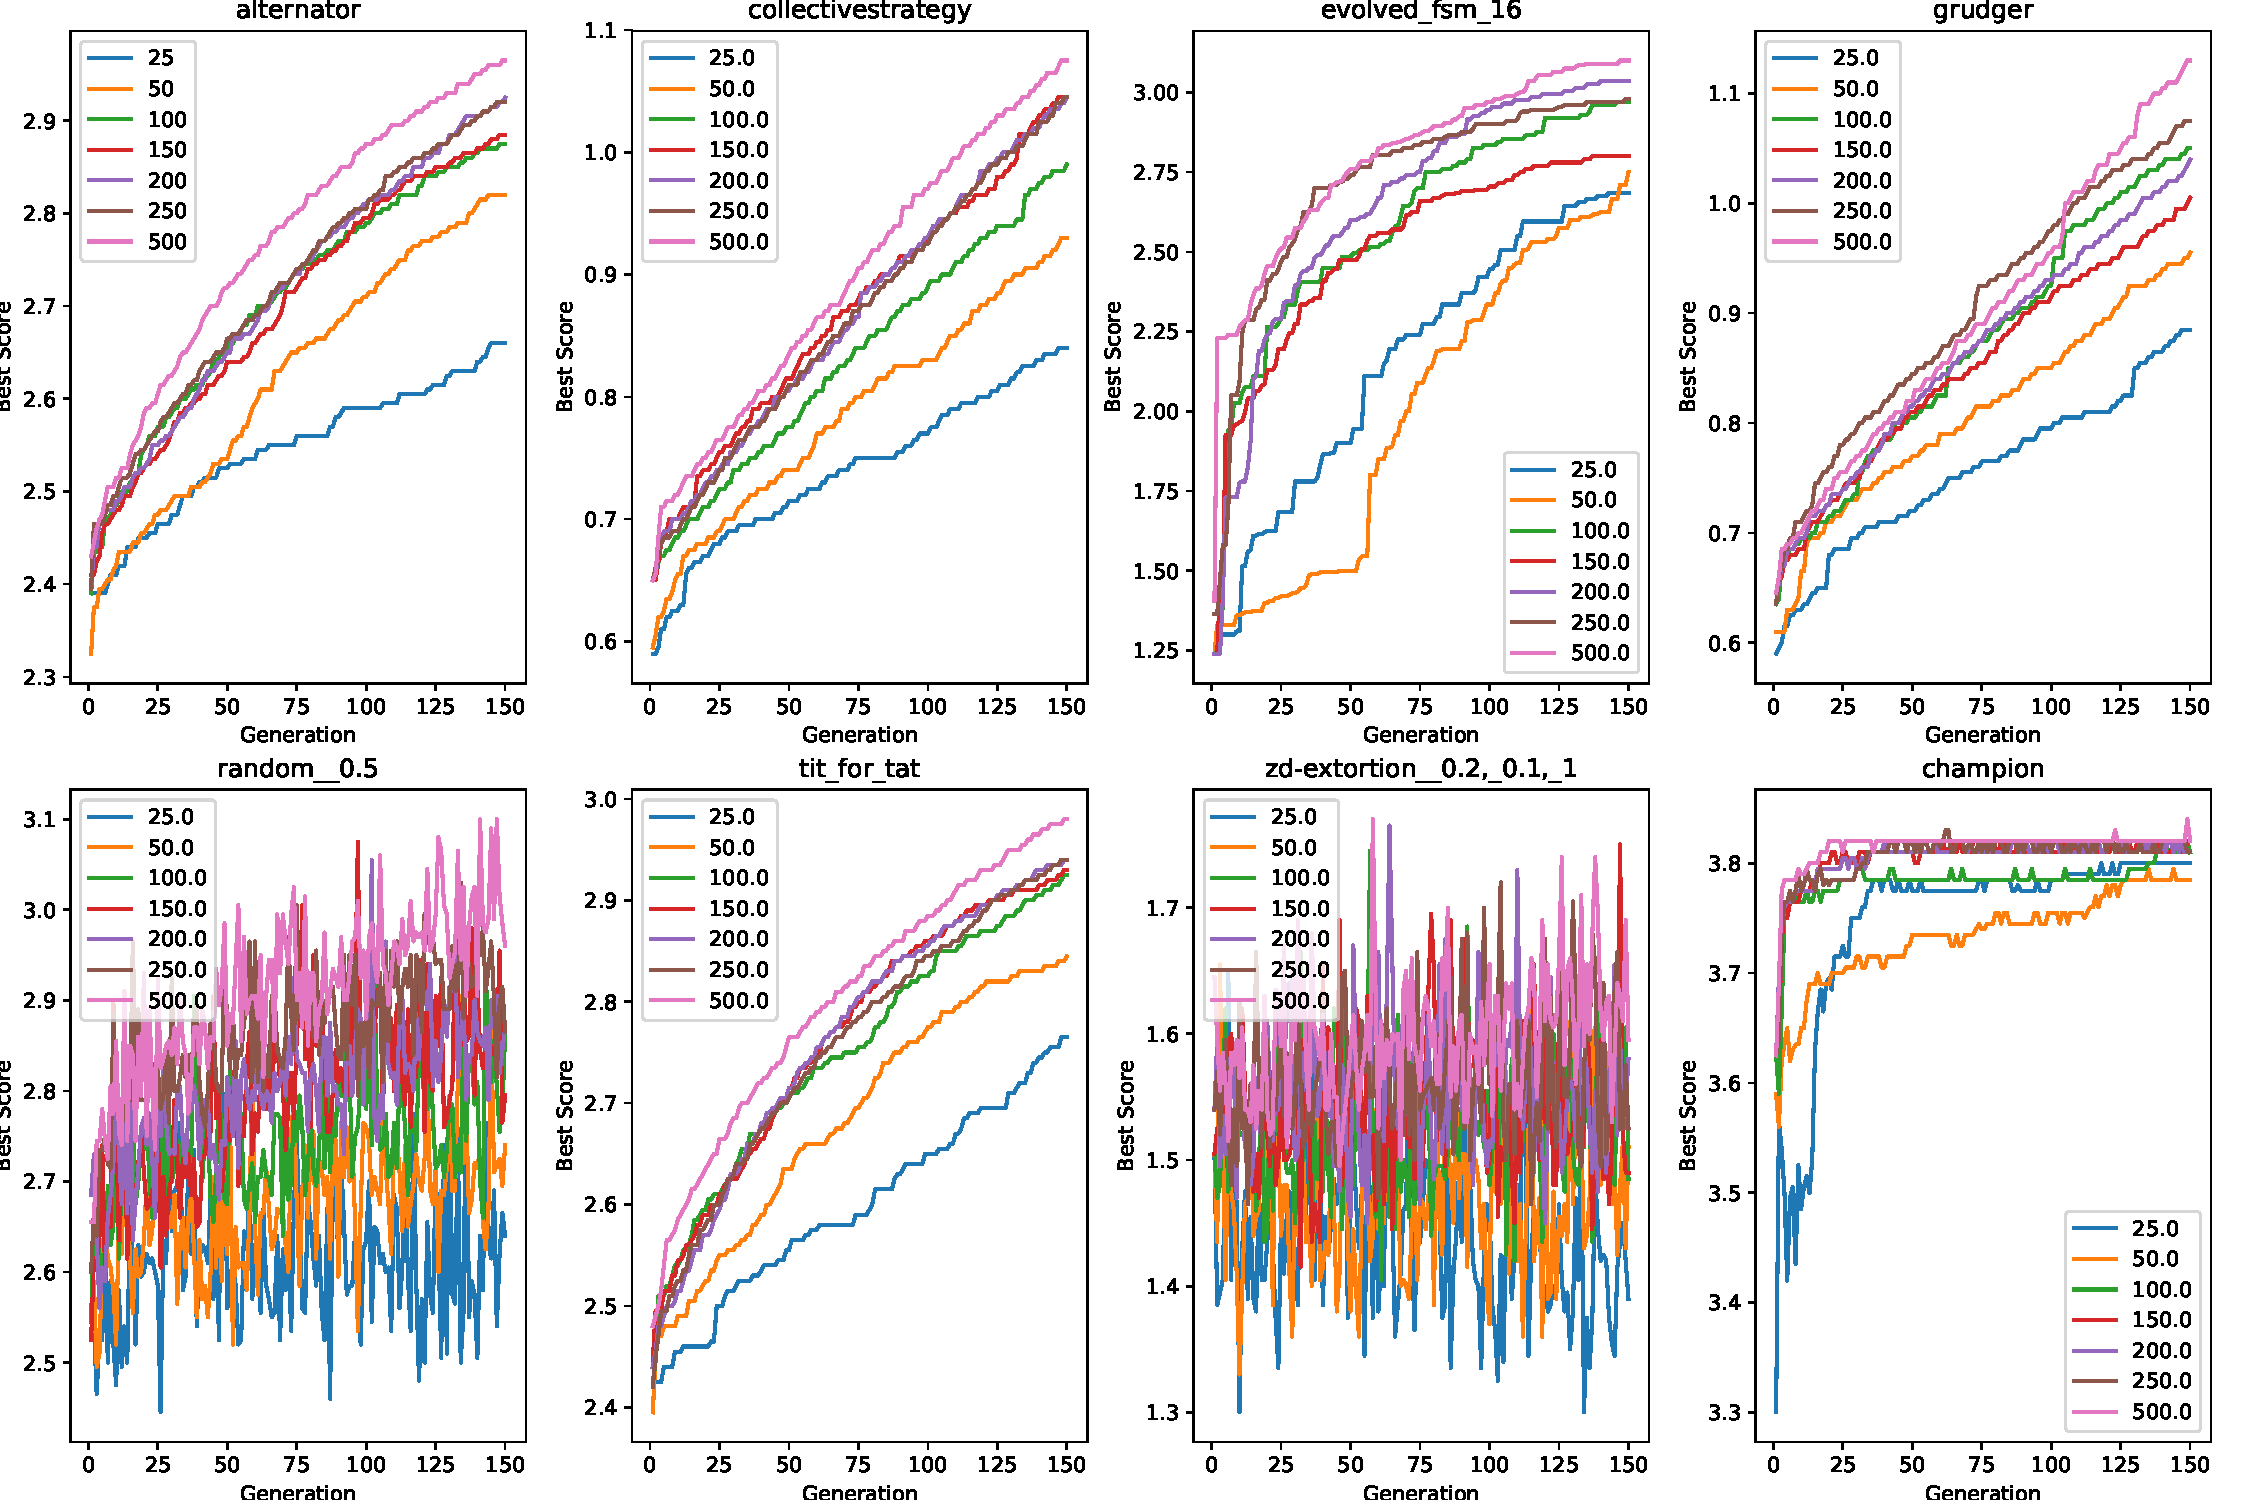
\includegraphics[width=1.0\textwidth, center]{./img/plots/INIT_POP_bs_v_gens_all.pdf}
    \caption{Best score per turn vs generation for different initial population sizes}\label{fig:INIT-POP-bs-v-gens-all}
\end{figure}

By grouping this data by the population we observe how initial populations affect different opponents.
Its clear that from figure~\ref{fig:INIT-POP-bs-v-gens-all} that the initial population size has a significant effect on finding better sequences.
We can see if there is a larger initial population there is typically a higher best score shown once concluding all of the generations.
This can also be shown in figure~\ref{fig:INIT-POP-mean-bs-v-init-pop-all} that\ldots
It doesn't, however, ensure that we find the solution sequence;
as is shown in the lack of long plateaus in the lines.\\

\begin{figure}[ht]
    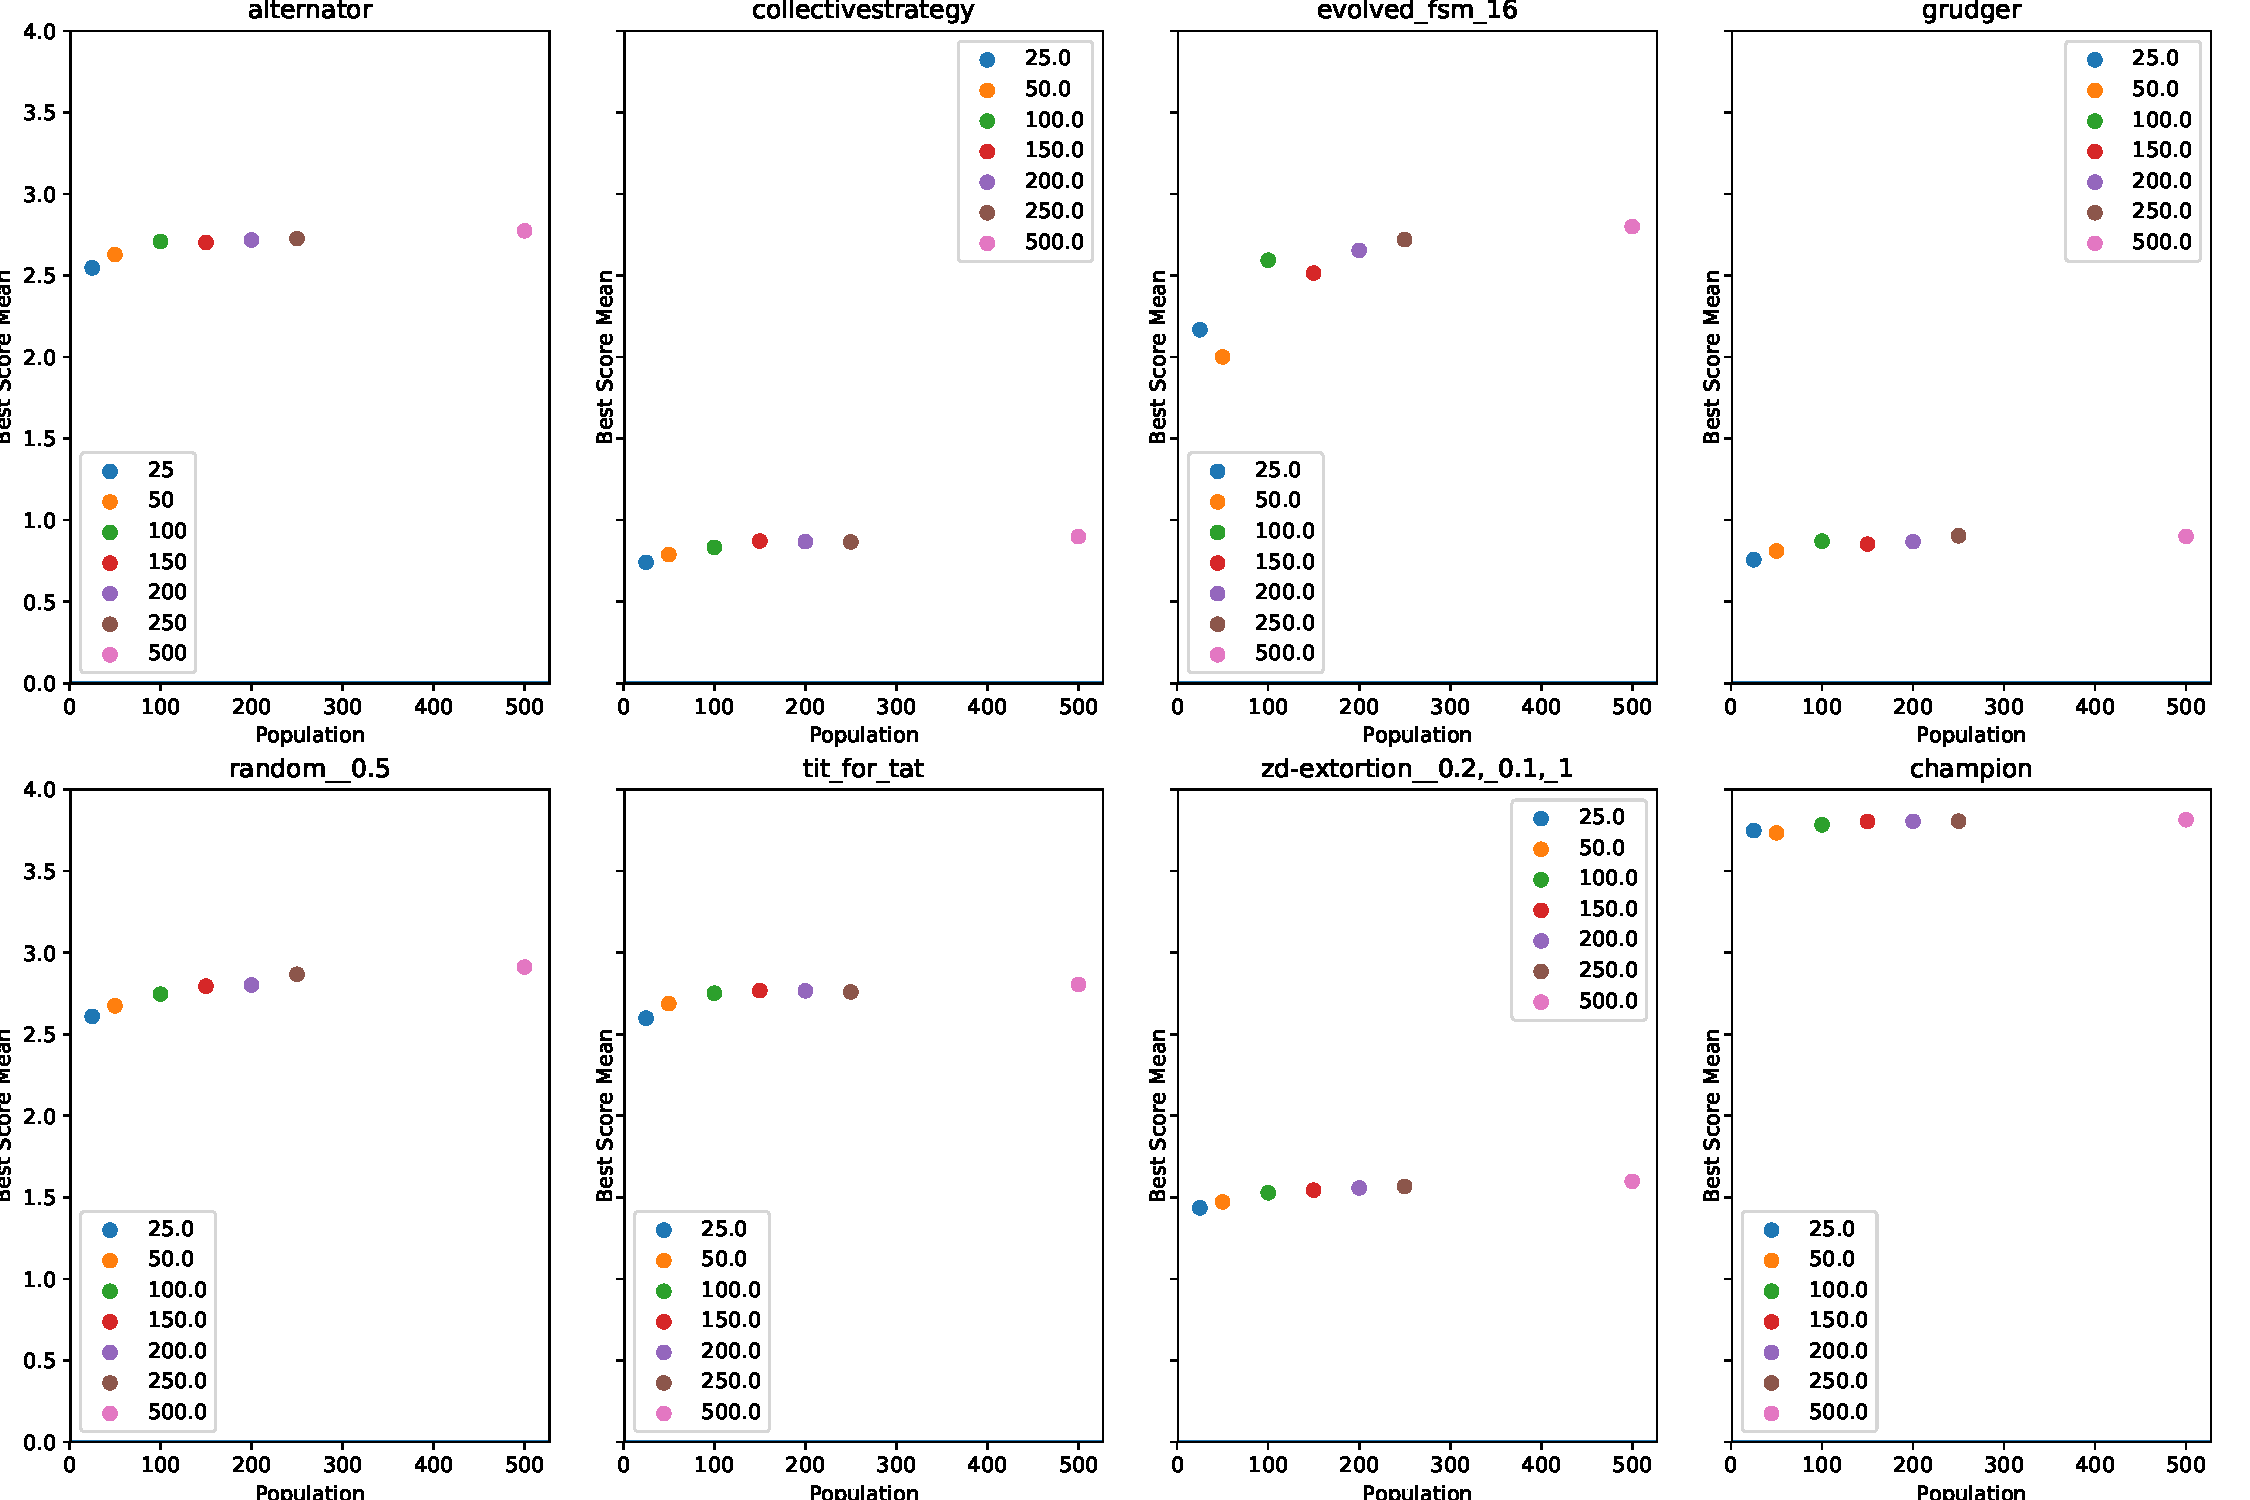
\includegraphics[width=1.0\textwidth, center]{./img/plots/INIT_POP_mean_bs_diff_v_init_pop_all.pdf}
    \caption{Scatter of max best score vs different initial populations}\label{fig:INIT-POP-mean-bs-v-init-pop-all}
\end{figure}

The improvement's from this effect are non-linear from observation.
The change in overall final best score for a population of 50 compared with a population of 100 is huge in comparison to the same relative increase from 200 to 250.
This may suggest there are more effective approaches to improving our score after a certain size of initial population than to continuing to increase it further.\\

% TODO:comment on each test opponent below?
% the RANDOM opponent tended to fare better with larger population, this may just be based on the probability that there is a sequence in the population that does better against the specific random sequence.
% This may also be the genetic algorithm optimising itself to the pseudorandom generator, building the \(Random()\) opponent solution for next generation, this could be a reason as all of the final generation best performers are scoring higher than the original starting population.
% the sequence is kind of converging to DDD...D, but there was no pattern for the algorithm to follow and so didn't converge.\\


None of these results have found a solution sequence (or at least we cant tell from the graph).
It is clear that larger initial populations do, on a relative scale, much better than small ones.
There are no large plateaus for the graph, so as we continue our research the initial population size will be increased to 150 to keep computation times manageable.\\

% TODO: another way of looking at effectiveness for initial pops?

\section{Generation Length Analysis}\label{sec:generationlengthanalysis}
Another major component parameter of a genetic algorithm is the number of generations it will run before outputting a final sequence.
The number of generations has an influence on a number of different things within the algorithm:

\begin{itemize}
    \item The total combinations of features, (sequence elements), that the algorithm can test.
    \item The number of low performers we can remove in our population.
\end{itemize}

For our goal of finding the optimal solution sequence for each opponent it would be useful to extend the generations as far as possible;
this would provide the most combinations of features possible.
Here we will look into how close to a solution sequence we get when we increase the generations the algorithm runs for.
Like in previous experiments with other variables we will use a set of sizes for our parameter to run our analysis for each size, here we will take generation lengths \(G \in [50,150,250,350,450,500]\).\footnote{We will be using a population of 150 as this was the best average for score vs computation time for analysis.}
The code in Snippet~\ref{code:generationChecker} shows how we will approach the analysis.\\

\begin{figure}
    \inputminted{python}{code_snippets/generationChecker.py}
    \caption{code to check multiple generation lengths.}\label{code:generationChecker}
\end{figure}

Generation size differs from other parameters in the fact this is purely performance based.
A genetic algorithm with 1 generation is just a series of tests;
with the results split into 2 sets --- winners and losers.
As we extend the generations we would be more focused on what happens to certain averages of results across the whole run, rather than absolute improvement.
If we look at figure~\ref{fig:GENS-mean-bs-diff-v-gens-all}, mean best score difference against the number of generations, we can observe how, on average, the number of generations has a declining effect the overall change in our best score per generation.\\

\begin{figure}[ht]
    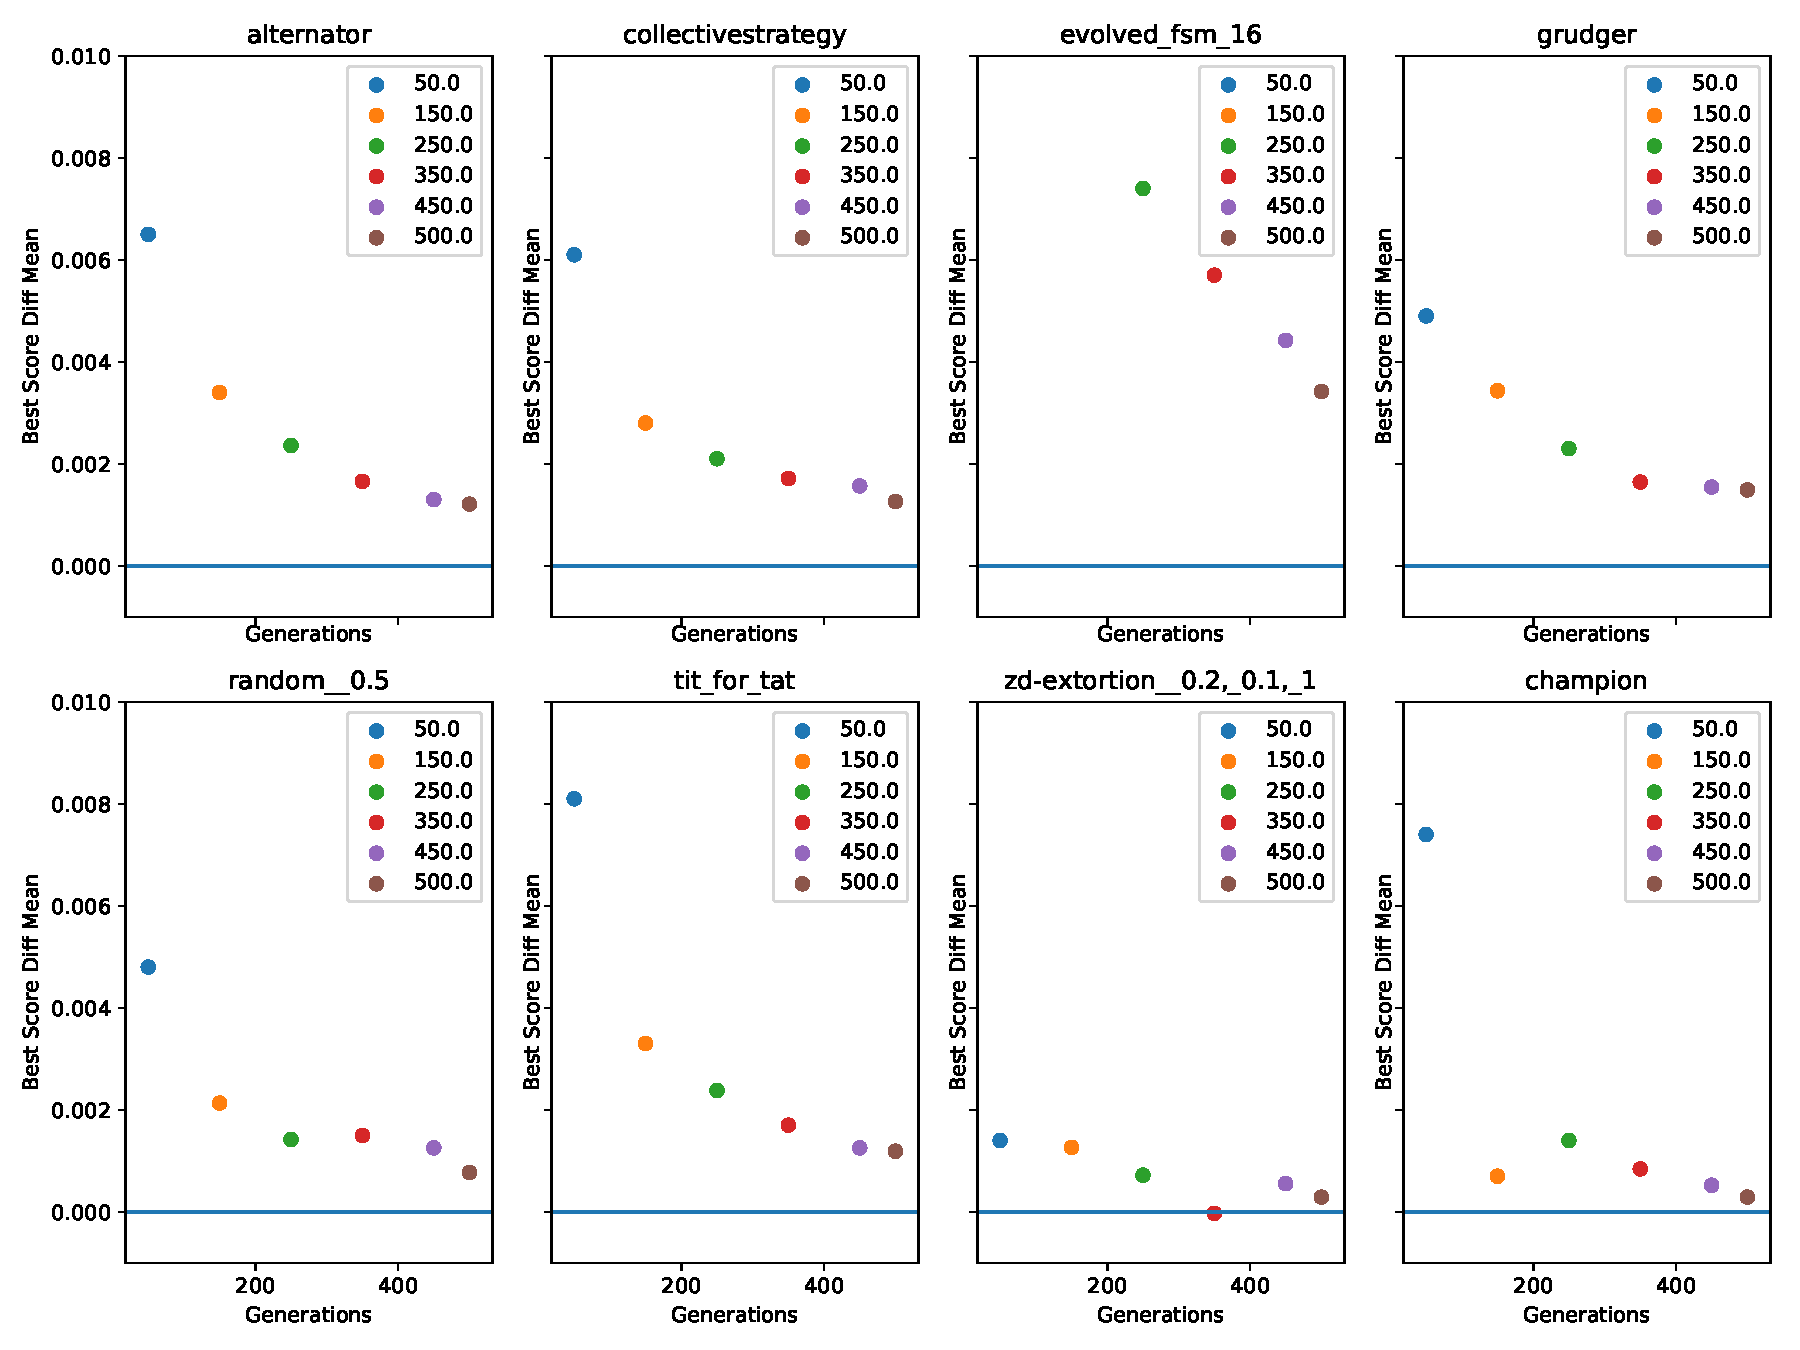
\includegraphics[width=1.0\textwidth, center]{./img/plots/GENS_mean_bs_diff_v_gens_all.pdf}
    \caption{Mean Best Score diff vs total generation lengths}\label{fig:GENS-mean-bs-diff-v-gens-all}
\end{figure}

This mean increase of score per generation trend is to be expected;
when we are close to a maximum it is more difficulty to randomly select which element in the sequence needs changing to improve our score.
On this result we can conclude as we increase generations there is less and less benefit per generation.
There is, however, still a benefit to extending the generations but we may have better performance by altering another parameter of the algorithm.
There may be a benefit from increasing the mutation rates when we get close to one of these maximums;
the more noisy our algorithm is for sequences could improve our chance of finding the correct solution.
The probably of finding a solution as we narrow in on a maximum decreases due to the number of elements that, when changed, will provide a better score.
Increasing the mutation frequency at this point means that there will be more members of the population that could potentially mutate the elements needed to improve the sequence.\\

Figure~\ref{fig:GENS-max-bs-v-gens-all} shows the proximity the optimal solution sequence once the analysis has concluded.
A good score is a score of 3 or more;
this can change from player to player, and is never explicitly obvious.
We can see that after a number of generations that solutions sometimes get `stuck' in a local maximum score.

% \begin{figure}[ht] 
% 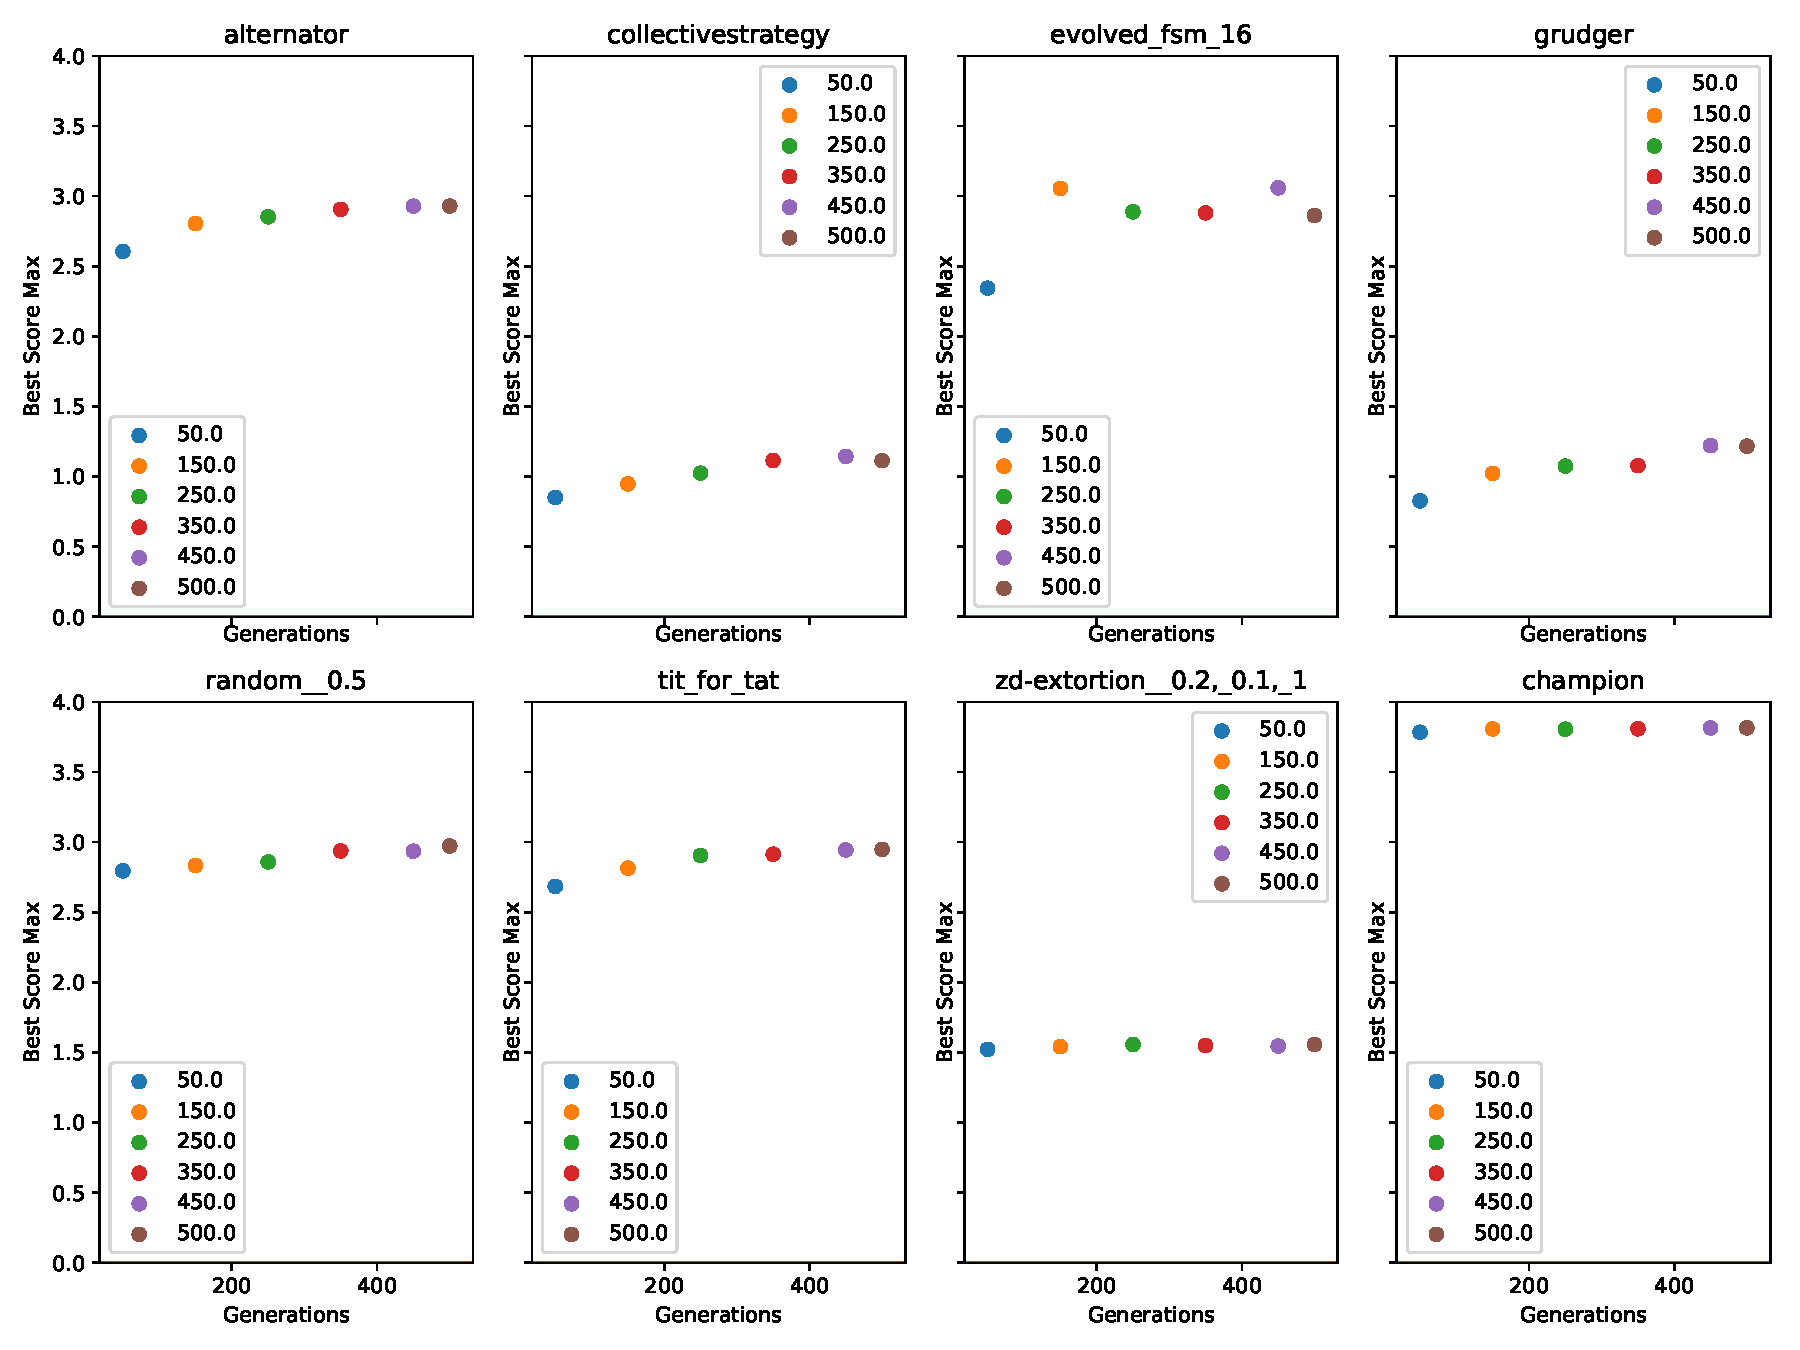
\includegraphics[width=1.0\textwidth, center]{./img/plots/GENS_max_bs_v_gens_all.pdf}
% \caption{Max best score vs total number of generations}\label{fig:GENS-max-bs-v-gens-all}
% \end{figure}

After 250 generations we \textit{seem} to have reached a solution state for our opponents Tit for tat and alternator but not for grudger.
Against Grudger we see an example, we have only reached an average score per turn of $\_\_\_$, which is obviously far from its optimal sequence.
From the combination of the plots, having more generations means that there is, on average, less of an improvement per generation.
It is clear that a higher number of generations is required to find a better solution sequence for an opponent.
From now on, 250 is the number of generations we will use to find our solution sequence during the analysis.\\

For most of the opponents 250 generations seems reasonable to reach a solution sequence as shown in the Alternator and Tit For Tat.
However, there are clear signs of local maximums occurring in the Grudger example.
Figure~\ref{fig:GENS-max-bs-v-gens-all} has reached a better sequence in 450 generations than 500\footnote{These are independent trials and have different sequences.}; meaning that increasing the generation length doesn't necessarily mean a local maximum.
The complexities with local maximums during the generations lie with mutation rates and crossovers.
We will cover this in Section~\ref{sec:mitigatingLocalMaximums}\\

In this investigation we will want to find the optimal solution and so, from these results, we will want to extend the generation length as far as possible.
An infinite number of generations would be preferable, but we don't have an eternity so a selection of a relatively large generation size will be adequate when coming to the final series of tests.\\

\section{Changing Mutation Rate}\label{sec:changeingmutationrate}
By changing the way in which we mutate our elements within a sequence, we might be able to more effectively narrow in on an optimal solution sequence.
The default settings are a frequency of 0.1; meaning for every 10 members of our population that continue into the next generation one of these has some elements in its sequence changed, and a potency of 1;
meaning that every sequence that was altered only has 1 element altered.
Here we will look into these 2 different concepts and see how they might improve our distance to an optimal sequence and whether we can escape local maximums.
\begin{itemize}
    \item Is it beneficial for more/less than 1 in 10 members to be mutated generation to generation? (More frequent mutation)
    \item Is changing one or more actions of a members' sequence the best way of mutating a candidate (More potent mutation)
\end{itemize}

These are two separate questions, so first we will look at increasing the potency of our mutation.
Once we have found some information on how this effects our solution, we can look into the frequency of our mutations with the new potency as a permanent setting.
As shown further on, there is not much of an improvement on our algorithm to changing either of these.The mutation algorithm is shown in Snippet~\ref{code:mutateFromDojo}\\

\begin{figure}
    \inputminted{python}{code_snippets/mutateFromDojo.py}
    \caption{The mutation code as given in the axelrod-dojo}\label{code:mutateFromDojo}
\end{figure}

EFFICIENCY NOTE\@: This approach allows for an \(O(1)\) factor of scaling.
This makes changes in mutation a great candidate for an approach to reduce our solution sequence distance compared with other approaches, for example increasing the population size.\\

\subsection{Changing Mutation Potency}\label{subsec:changingMutationPotency}
Changing the potency of the algorithm will mainly generate the noise in our sequence generation to generation, increasing the distance\footnote{Distance concept has been taken from coding theory; \(d(s_1,s_2)\) = the number of differing positions between 2 sequences \(s_1\) and \(s_2\).
For example: \(d(111,110) = d(CCC,CCD) = 1 \)} between the mutated sequence from the original.\\

This potentially could create an algorithm that is too `jumpy' for narrowing in on a solution.
We can imagine a sequence as a vector in 200 dimension space then a mutation for element \(S_i\) is the same as changing the vector in its \(i^th\) dimension.
Shortening this example to a vector in 3 dimensions (or a sequence of length 3) then a mutation is much more easily visualised.
It is clear that a mutation potency should be kept low as to keep consecutively mutated sequences more similar;
we will only be looking at mutating our sequences at up to 10 percent of their elements.
We will look into having mutation potencies \(M_p \in [1,2,3,5,10,15,20]\)\\

\begin{figure}
    \inputminted{python}{code_snippets/mutationPotencyChecker.py}
    \caption{Mutation potency code}\label{code:mutationPotencyChecker}
\end{figure}

Using the data generated from Snippet~\ref{code:mutationPotencyChecker} of code we are able to look at how our best score and our best score diff is affected as we increase the number of positions.\\

\begin{figure}[ht]
    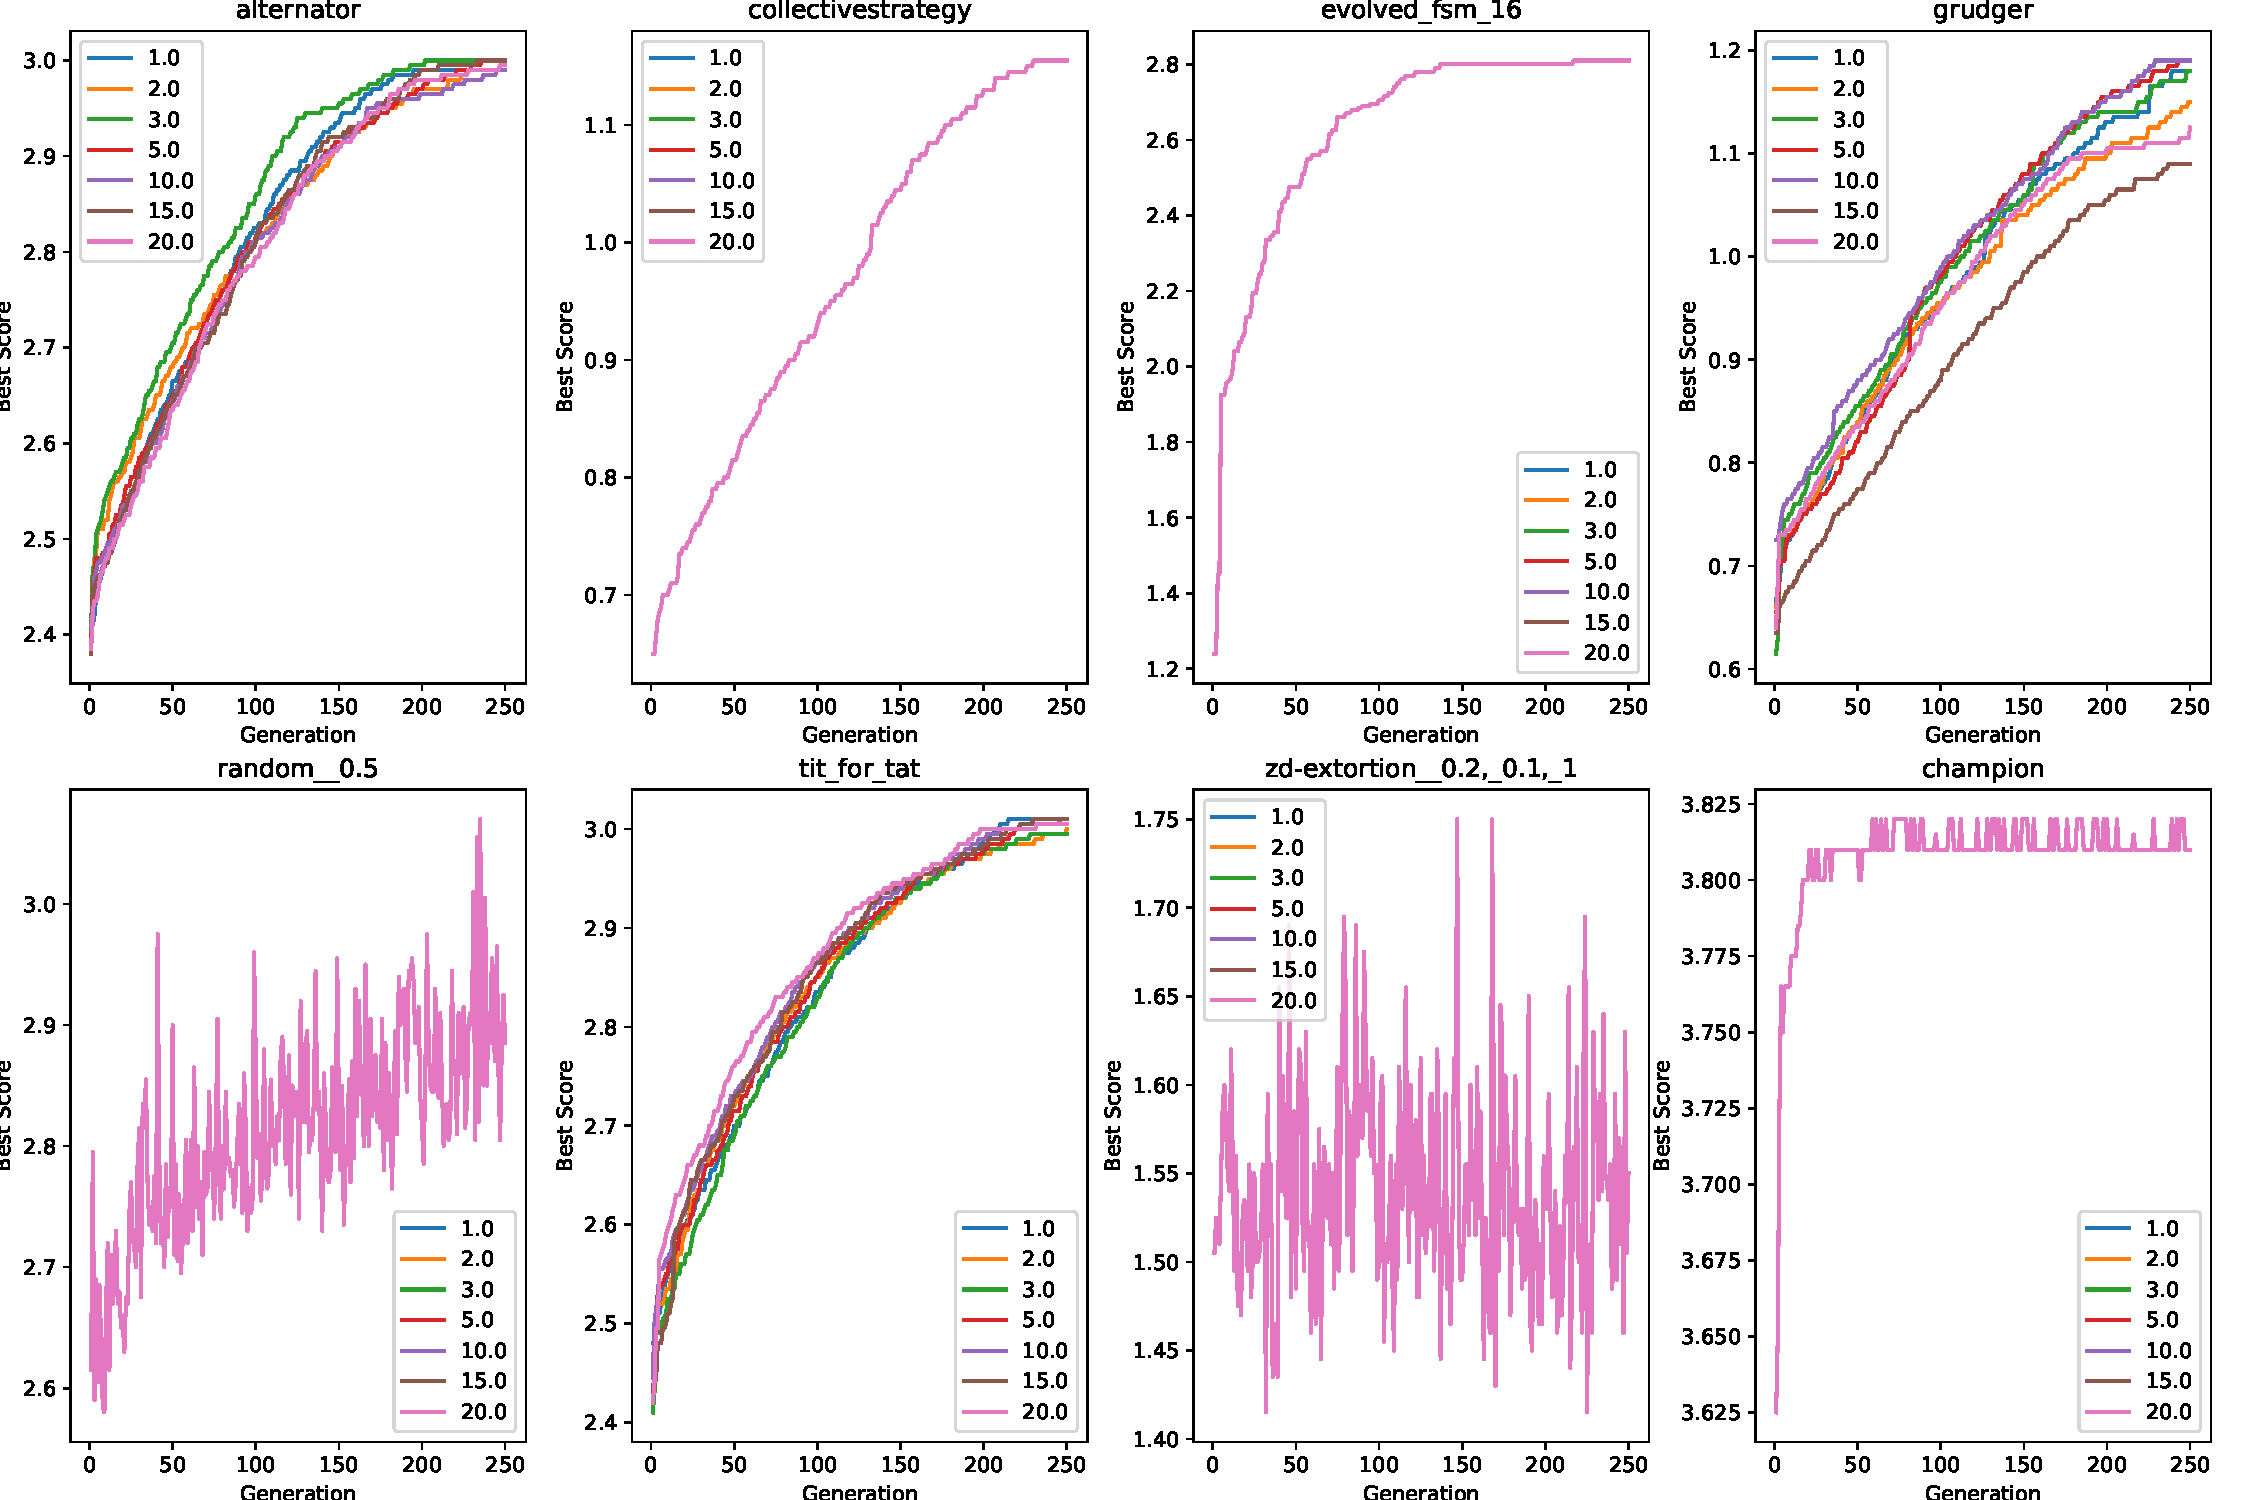
\includegraphics[width=1.0\textwidth, center]{./img/plots/MUT_POT_bs_v_gen_all.pdf}
    \caption{Best score vs generation for different mutation potencies}\label{fig:MUT-POT-bs-v-gen-all}
\end{figure}

Figure~\ref{fig:MUT-POT-bs-v-gen-all} shows no clear benefit from increasing the mutation potency.
We can see that having changed 15 genes in our sequence each time we are still not improving our score as much as changing only 1.
This may be down to chance (and if the test is rerun this may disappear), however looking at more opponents than just Grudger we find there is no clear benefit to increasing the mutation potency with respect to the overall best score value against an opponent.
If we instead look at what our average increase of score per mutation is we may observe a useful result.\\

\begin{figure}[ht]
    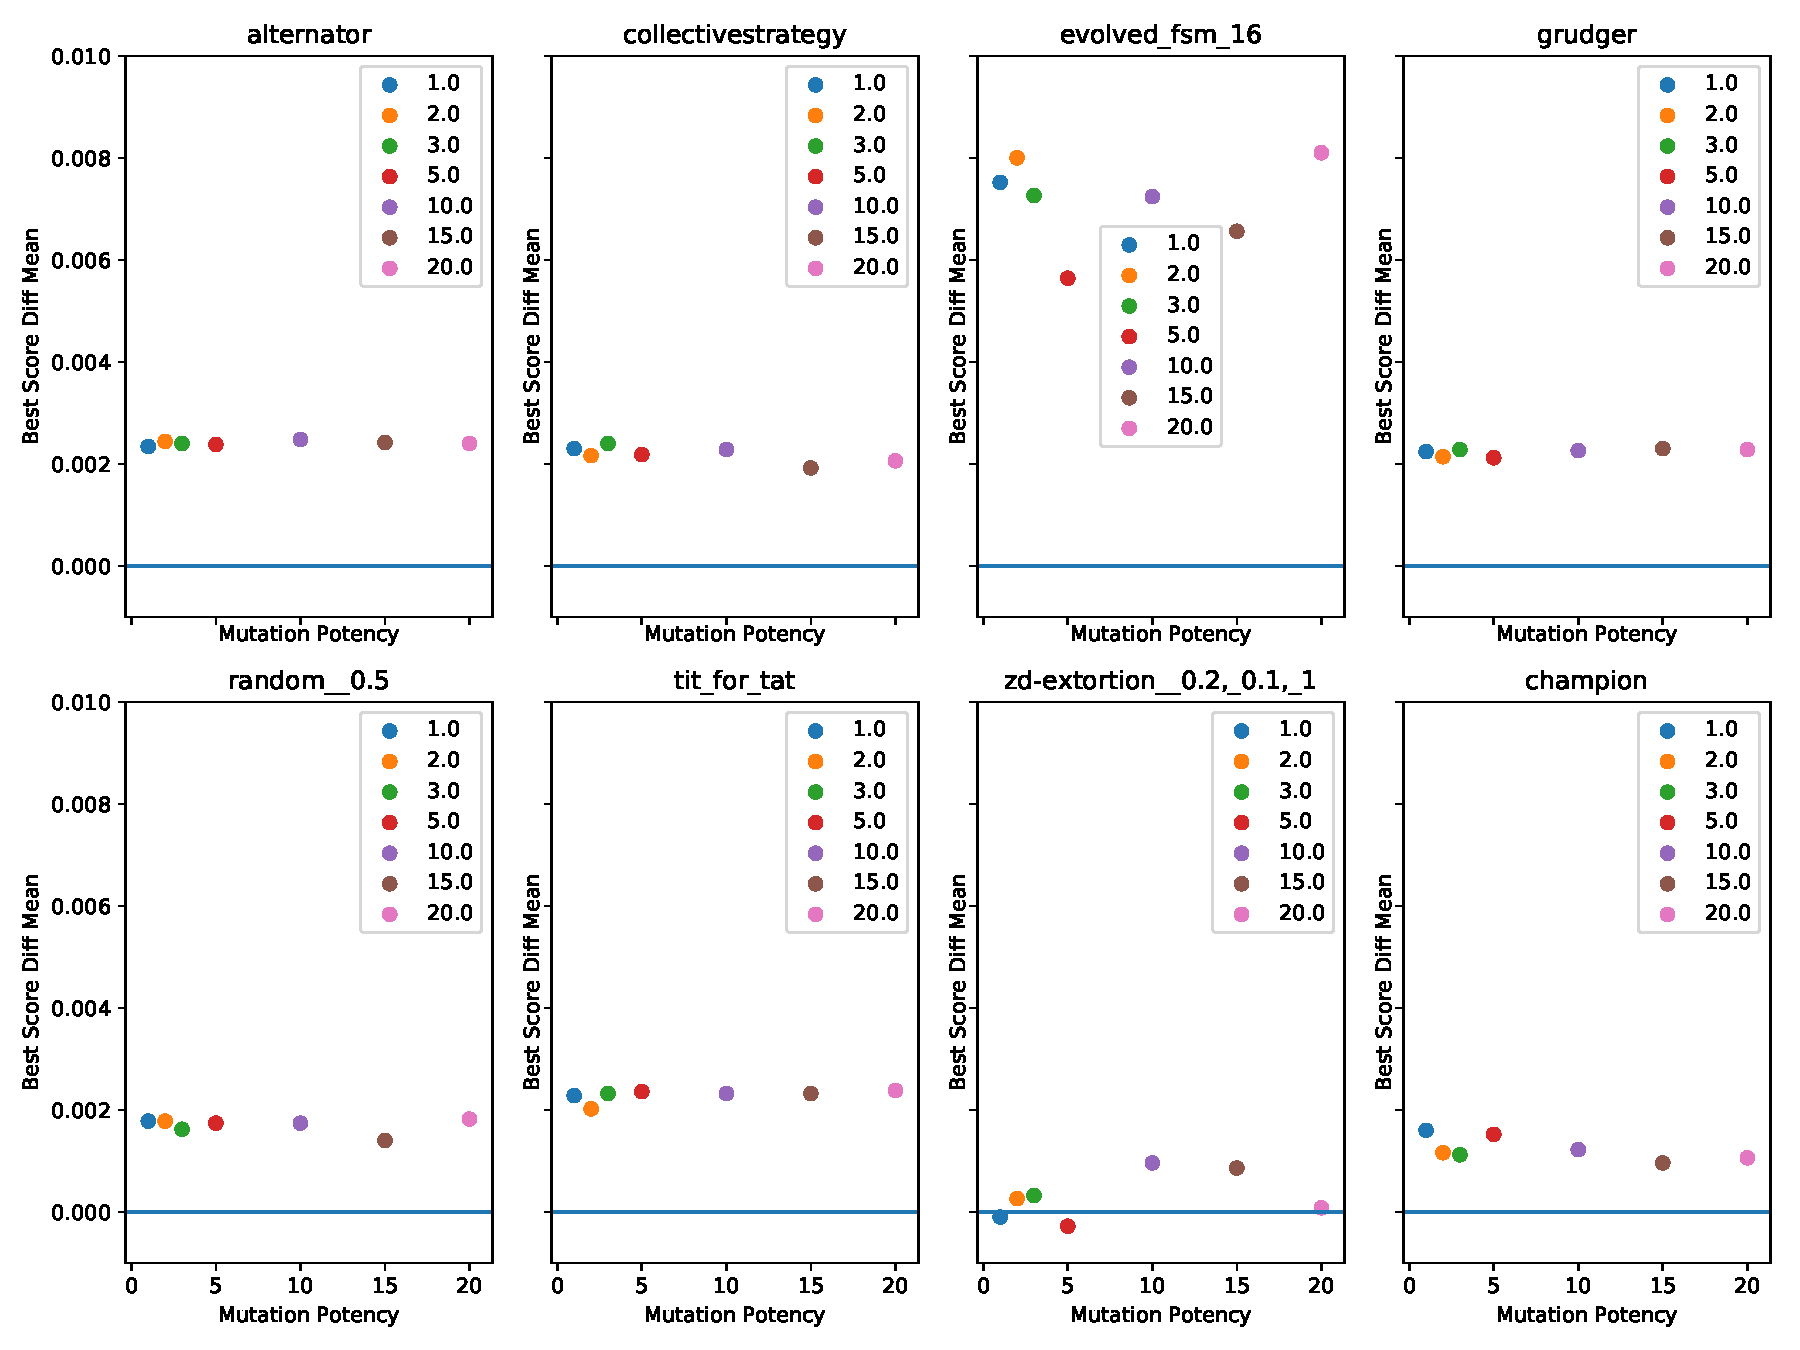
\includegraphics[width=1.0\textwidth, center]{./img/plots/MUT_POT_bs_diff_v_pot_all.pdf}
    \caption{Average best score diff vs mutation potencies}\label{fig:MUT-POT-bs-diff-v-pot-all}
\end{figure}

From looking at how our average best score difference changes as we increase the mutation potency there is no sign that there is a significant improvement to our sequence.
The increase in mean best score difference is not substantial and could be down to chance.

\subsection{Changing Mutation Frequency}\label{subsec:changingMutationFrequency}
In contrast to changing the mutation potency, increasing the frequency should allow us to generate more unique sequences generation to generation.
We will look at what happens when we run the genetic algorithm on a set of mutation frequencies \(M_f \in [0.1,0.2,0.3,0.4,0.5]\).
The code in Snippet~\ref{code:mutationFrequencyChecker} shows the algorithm that will complete this analysis.\\

\begin{figure}
    \inputminted{python}{code_snippets/mutationFrequencyChecker.py}
    \caption{Mutation potency code}\label{code:mutationFrequencyChecker}
\end{figure}

\begin{figure}[ht]
    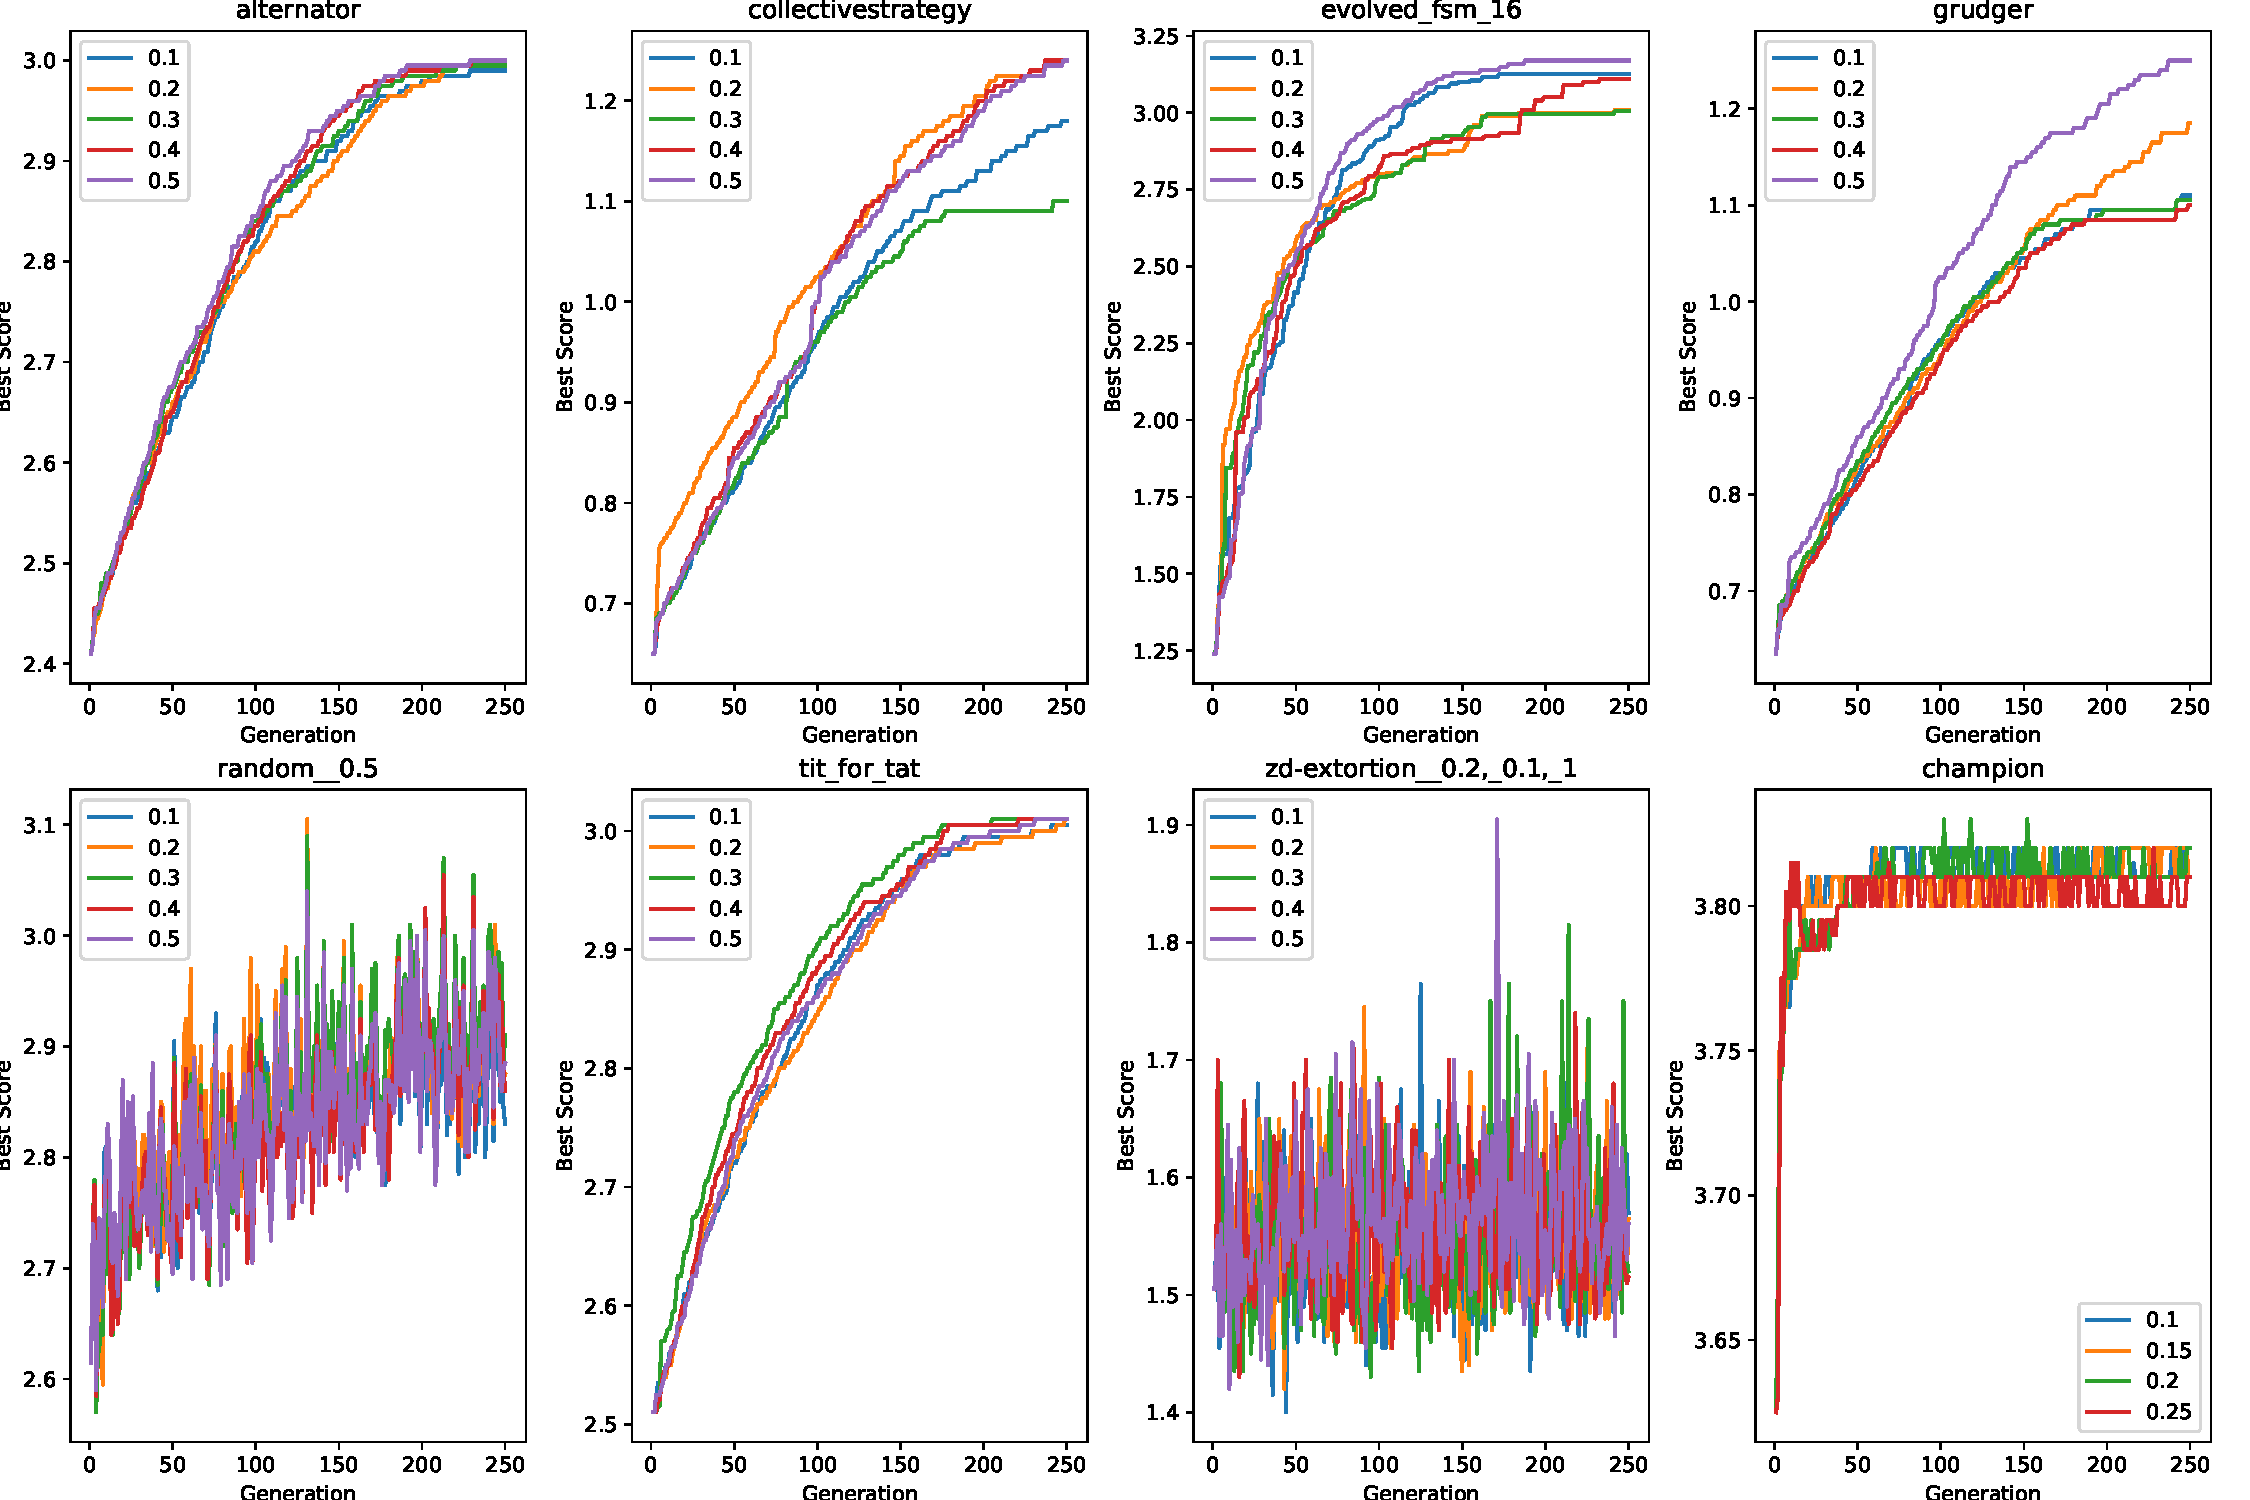
\includegraphics[width=1.0\textwidth, center]{./img/plots/MUT_FREQ_bs_v_gen_all.pdf}
    \caption{Best score vs generation for different mutation frequencies}\label{fig:MUT-FREQ-bs-v-gen-all}
\end{figure}

The results on changing the mutation rate don't obviously effect that generations until convergence from this overview.
There is an interesting result that can be seen on the grudger plot;
the algorithm has found 2 different maximums.

\begin{figure}[ht]
    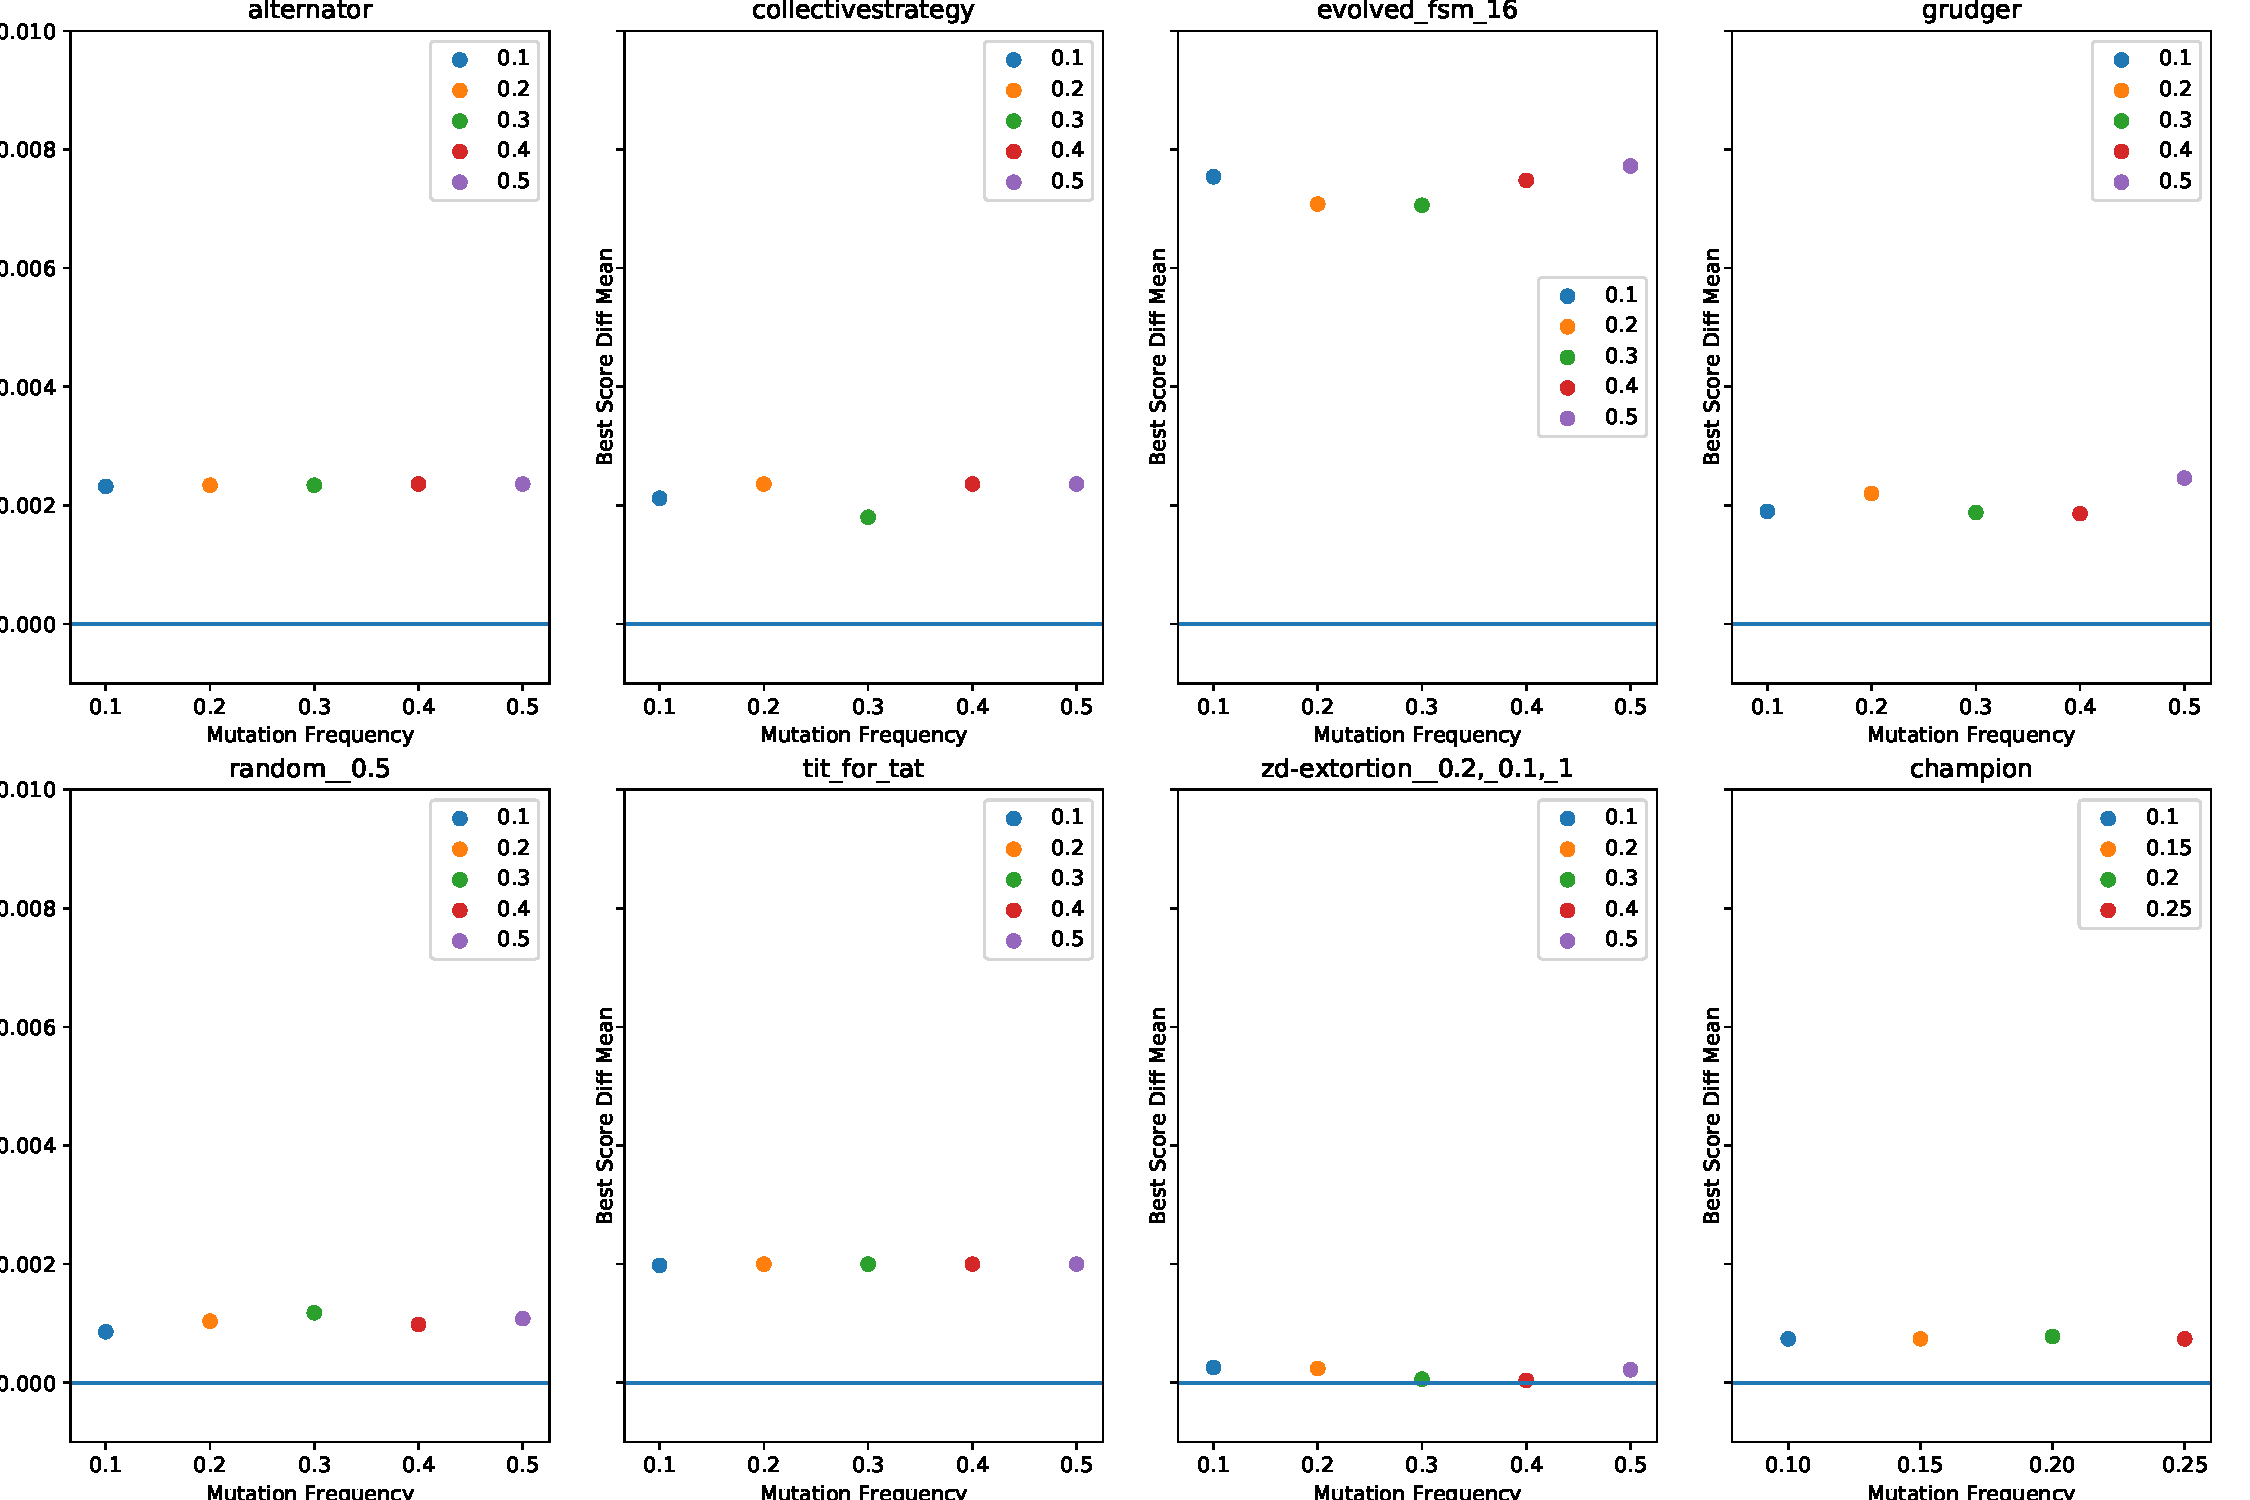
\includegraphics[width=1.0\textwidth, center]{./img/plots/MUT_FREQ_bs_diff_v_freq_all.pdf}
    \caption{Average best score diff vs mutation frequencies}\label{fig:MUT-FREQ-bs-diff-v-freq-all}
\end{figure}

From Figure~\ref{fig:MUT-FREQ-bs-v-gen-all} we can see that the mutation frequency of 0.1 and 0.2 produced higher scoring solutions than the other mutation frequencies.
This shows that we have found 3 different solution sequences (in freqs .15, .2, .25) with the solution for .1 continuing to improve as the generations ended.\\

As an additional point, we can also observe that increasing the mutation frequency means that there is less variation in the best scoring sequences.
%  (TODO: Does this have an impact on escaping local maximums?)

\section{Mitigating local maximum solutions}\label{sec:mitigatingLocalMaximums}
The occurrence of local maximums is something that has only occurred in sequences against for the Grudger opponent so far.
Figure~\ref{fig:MUT-FREQ-bs-v-gen-all} shows that there are clearly 2 distinct plateaus that are reached in terms of score, and the overall scores are much lower than the optimal, around \(1.4\).\\

The difference between the Grudger and the other opponents have been looking at is that the Grudger has a singularity point where its behaviour changes.
The change in behaviour is not uncommon, Tit For Tat works in a similar way and in both cases our algorithm has managed to identify this behaviour and adapt to overcome its negative effects.\\

Grudger is an opponent which it is possible to attain a local maximum score and be `trapped' in this solution sequence.
From the output sequences below it appears that the sequence is being changed into becoming 2 sections of opposing moves.
If we look at a random start sequence and then the end sequence after 250 generations we can see that the genetic algorithm is learning defect after some point and cooperate before.
This is due to the fact a good solution will end in lots off defections after it has already defected, but cooperate beforehand to avoid this harsh behaviour.\\

%Grudger best start: \(C:[6,8,2,1,2,1,6,1,2,2,4,2,1,1,2,10,1,1,1,3,1,3,1,1,1,1,2,2,1,1,1,2,3,5,2,2,2,1,1,2,1,1,4,1,2,1,1,1,2,3,1,1,2,2,1,7,3,2,1,2,3,1,1,5,1,1,1,1,1,1,1,1,1,1,4,1,1,1,1,4,2,1,1,3,1,1,2,3,4,1,1,3,2,4,2,1,2,3]\)\\
Grudger best start: CCCCCCDDDD\ldots (No pattern is obvious.)

Grudger best end: \(C:[22,178]\)\\

We may be able to identify a way to mitigate this singularity effect by looking at the difference between 2 similar solutions.
Grudger and Tit For Tat differ in their strategies in two ways:

\begin{itemize}
    \begin{item}
        Grudger never changes its mind.
        There is one change in behaviour for the entire game, unlike Tit For Tat.
        The algorithm then only has a single opportunity to observe this per population per generation meaning the behaviour is much less frequently encountered.
    \end{item}
    \begin{item}
        Grudger will not become `smart' again.
        This means that the move genetic algorithm picks up the effect of a single defection in its sequence it starts playing a `dumb' opponent.
        A random start of Cs and Ds puts the likeyhood of at least 1 defection occurring in the first 10 moves at above \(99.99\% \).
        This swap from `smart' to `dumb' will, most likely, always occur in the first 10 moves;
        the only way of extending the `smart' player is to add a cooperation to the end of the starting Cs.
    \end{item}
\end{itemize}

Snippet~\ref{code:gudgerTotalities} shows two totality games against grudger, one of all Cs and one of all Ds.
These are edge cases and would be incredibly rarely encountered as a starting point in the random initial population.
Because of this, the algorithm has to shuffle towards the potential benefit of using these totalities rather than start with analysing them.
Our case against grudger requires the algorithm to attempt this shuffle towards a totality after encountering the grudging effect.
This would then require the algorithm to select (using random selection out of 200) the first defection move and change it (only 1 in 10 members are mutated) to a cooperation move.
This likelihood is incredibly small, and starting at common or uniform sequences would be more beneficial, as posed in Section~\ref{sec:alteringinitialpopulation}.\\

\begin{figure}
    \inputminted{python}{code_snippets/grudgerTotalities.py}
    \caption{Grudger matches against totalities}\label{code:gudgerTotalities}
\end{figure}

% TODO: need this para? I feel like I'm repeating myself
As Snippet~\ref{code:gudgerTotalities} shows, we should be converging on a totality of Cs rather than what its doing;
finding the totality of Ds.
This is probably because the algorithm initially limits its best score per turn once the first generation is complete and a cut-off has been established for each of the initial population.
The crossover method between generations then doesn't provide enough of a mix up to allow the algorithm to escape the local minimum by switching a subsection with a sufficiently different potentially better subsection.
Then when it comes to mutating, there is little any number of mutations can do to drastically change large sections of the sequence without having a huge effect on the score.\\

\subsection{Ineffective Approach of Altering Crossover And Mutation}\label{subsec:ineffectiveApproachOfAlteringCrossoverAndMutation}
The process of converging to Ds when building a solution against grudger then sheds light on the process the algorithm takes to find a solution.
If we are to find the optimal solution sequence, we must take a crossover and mutation path which doesn't cut off better paths as we work our way towards good solutions;
this is much easier said than put into practice due to the way the algorithm `cuts off paths'.
If we reverse this thinking and try to alter our crossover design and mutation rate such that instead of `cutting off' a path we are able to `build' new ones.
We can re-design the crossover to switch up large subsections of the sequence then allow the mutations to optimise these sub-sequences.\\

Currently we have the following design:
\begin{figure}
    \inputminted{python}{code_snippets/oldCrossover.py}
    \caption{Old Crossover algorithm}\label{fig:oldCrossover}
\end{figure}

% TODO: look into tikz
We want to allow the crossover to have more of an impact than just halving the sequence and optimizing each section.i.e.go from:\\
\[|--------------------| and |++++++++++++++++++++|\]
\[= |----------++++++++++|\]
to the mixture:\\
\[|--------------------| and |++++++++++++++++++++|\]
\[= |--++--++--++--++--++|\]\\
This will allow the mutation rate to edit the subsections in a more interlaced manner, hopefully overcoming the pitfalls of sparse mutations to escape local maximums.
Our new crossover method is shown in Figure~\ref{fig:newCrossover}.
As shown, the algorithm splits the two sequences into 10 section and the new sequence is formed from Alternating sections.
Figure~\ref{fig:newCrossoverEX} shows an example of the new crossover method.\\

\begin{figure}
    \inputminted{python}{code_snippets/newCrossover.py}
    \caption{New Crossover algorithm}\label{fig:newCrossover}
\end{figure}

\begin{figure}
    \inputminted{python}{code_snippets/newCrossoverEX.py}
    \caption{Example of new crossover algorithm}\label{fig:newCrossoverEX}
\end{figure}

We will look at how this new crossover algorithm works with the default mutation (freq=.1 and pot=1) to improve our local maximums with the selection off opponents.\\

There was no noticeable improvement from introducing this change of function.
Each players average score per turn was in the expected score if the algorithms crossover method was unchanged.
The problem of mitigating sub optimal solutions may be more efficiently solved using a predefined population.
Section~\ref{sec:alteringinitialpopulation} discusses this in more detail.

\section{Altering Initial Population}\label{sec:alteringinitialpopulation}
Altering the initial population allows us to select starting sequences that fit patterns we know will have good results.
For example totalities, with heads/tails, are usually very effective against simple opponents;
for example Tit For Tat, `dumb' opponents or Grudger.
Alternating and certain known solution optimal sequences are good starting sequences for an initial population, allowing a more intelligently distributed set of starting points for the random mutation process.\footnote{This can be visualised as placing balls on a `lumpy' 2d plane to try and find the minimum, starting with an educated guess means we wont get all the balls stuck in one vally which isnt the deepest.}

This section discusses the results of working on an initial population that contain common solution sequences.
We will start by creating a population of `neat' starting members then allow the entropy of the genetic algorithm to alter these sequences.
Deciding where to start our algorithm may mitigate potential sub-optimal solutions by reducing the distance between the starting sequences and optimal solutions.
The list of `neat' starting points are stated below:\\

Totalities
\begin{itemize}
    \item \(C:[200]\) | 1 sequence
\end{itemize}

Single Change Sequences
\begin{itemize}
    \item \(\{C:[i,200-i]\} \quad i\in [1,10],\ i \in \mathbb{Z}\) | 10 sequences
    \item \(\{C:[200-i,i]\} \quad i\in [1,10],\ i \in \mathbb{Z}\) | 10 sequences
\end{itemize}

Matching Tail Sequences
\begin{itemize}
    \item \(\{C:[i,200-(i+j),j]\} \quad i,j \in [1,5],\ i,j \in \mathbb{Z}\) | 25 sequences
\end{itemize}

Alternating
\begin{itemize}
    \item \(C:[\ (i,i)^{100/i}] \quad i \in \{1,2,4,5\}, i \in \mathbb{Z}\) | 4 sequences
\end{itemize}

Handshakes
\begin{itemize}
    \item \(C:[\ i,j,k,200-(i+j+k)] \quad i,j,k \in \{0,1,2,3\}, i \in \mathbb{Z}\) | 4 sequences
\end{itemize}

For each of these sequence sets the inverse, with a defection move start, will also be added to the set of starting sequences.
This in total gives 164 (after code~\ref{code:initialPopulationCode}) of sequences, we will then make up the difference to the population limit using a set of random sequences.\\

We can now look into how this has effected the previous experiments.

\subsection{Population Size}\label{subsec:populationSize}

\begin{figure}[ht]
    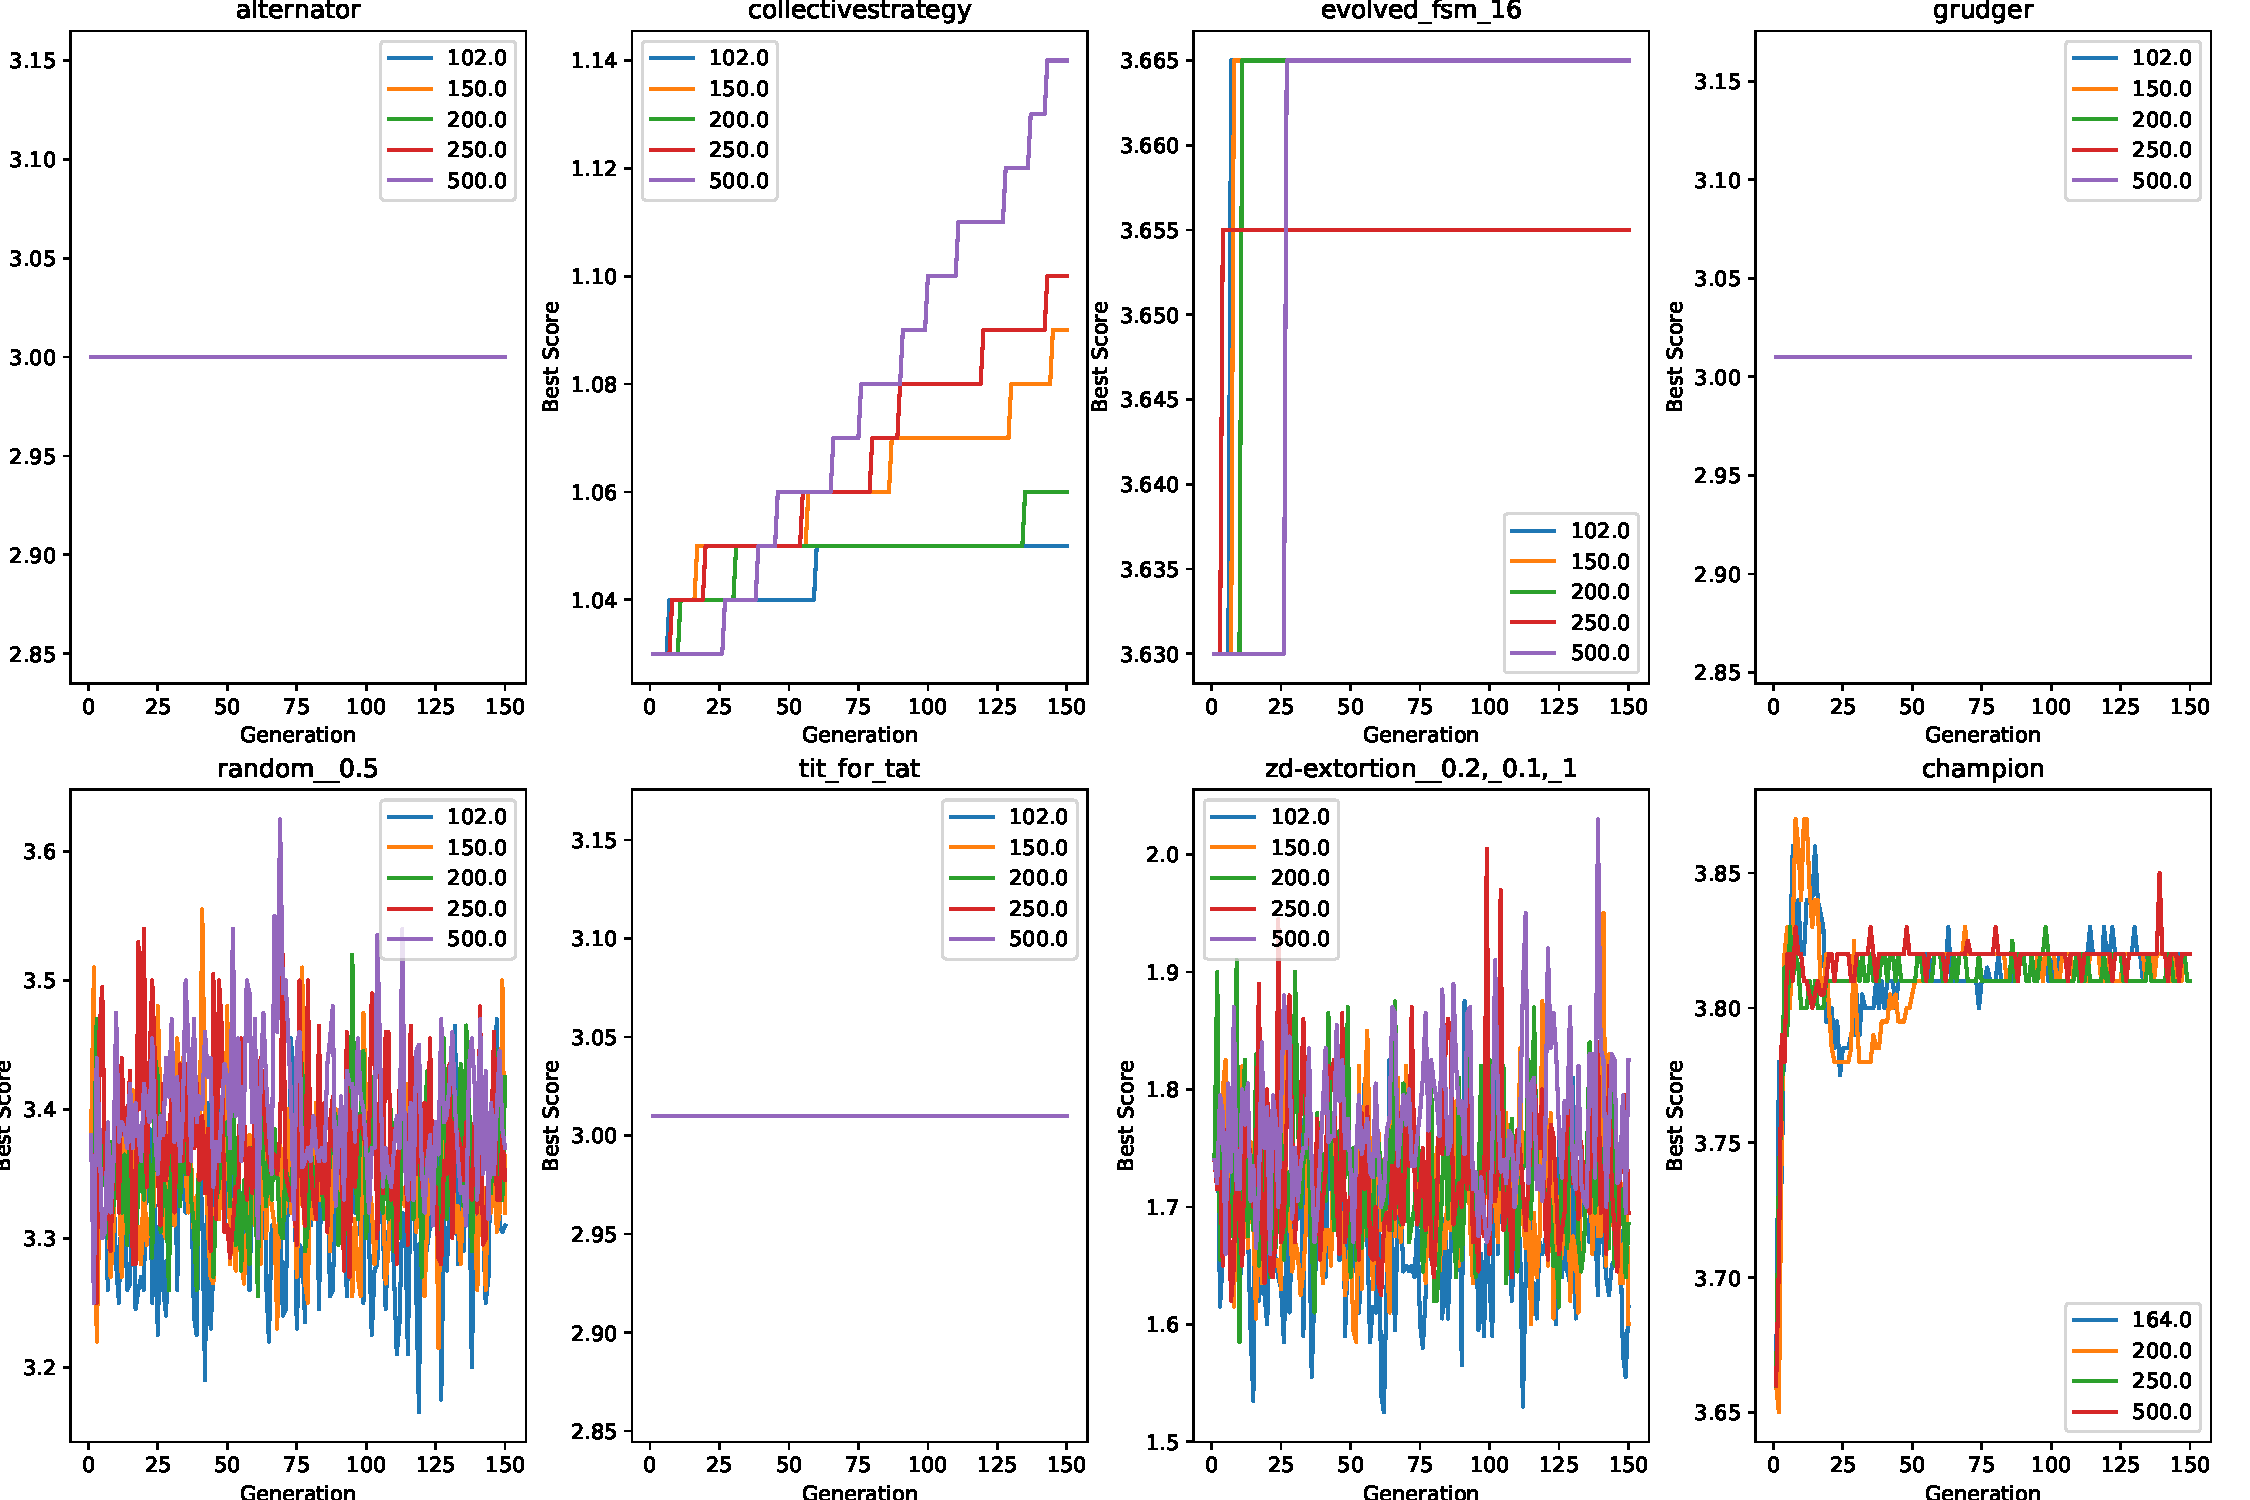
\includegraphics[width=1.0\textwidth, center]{./img/plots/NEW_INIT_POP_bs_v_gen_all_old.pdf}
    \caption{Best Score vs generations for preset initial populations on top of random sequences}\label{fig:NEW-INIT-POP-bs-v-gen-all}
\end{figure}

Figure~\ref{fig:NEW-INIT-POP-bs-v-gen-all} shows the results of using a given initial population of sequences of size 102 along with supplementing this with random members.
We will have \(|P| \in [102,200,250,500]\).
The Collective Strategy run in figure looks as if there are much better results with an initial set population for the algorithm.
Of the two that are not showing straight lines we can observe that the algorithm has found the optimal sequence for all but Random \& Collective Strategy.
This is probably due to 2 different reasons:

\textbf{Random}: The `dumb' strategy should being beaten with a totality of D, the algorithm has in fact converged to almost this totality, but still has intermittent Cs.
The reason for this is the scoring grade `score per turn' will reflect on the number of intermittent Cs in the Random players sequence.
More Cs in the Random sequence will allow the algorithm to score more.
This leads to a solution sequence containing some random Cs not because they score better in some turns, but because the totality of Ds played against
a Random sequence would `loose' to a sequence containing some Cs in because its not a fair trial;
the two sequences play against different Random opponent sequences.
\textbf{Collective Strategy}: as described in chapter~\ref{sec:strategiesOfInterest} this strategy is, basically, a handshake + Grudger.
If we look into the sequence it selected we can see its found the handshake but then arrives on Grudger.
After this encounter the same problem as we had before population selection occurs and the algorithms limits the damage by splitting into Cs then Ds.Solving the collective strategy (and handshakes in general) may be simple;
we just put in all the possible n move handshakes followed by totalities and then set to work on the 2nd part of the sequence.\\

It is clear that having a larger population is good from the old analysis, but the initial population still has to be tweaked to improve its scores against certain handshake opponents.
The Random opponent is a special case that requires more analysis to find the absolute optimal.
The new initial population, now of size 164, will include all combinations of C \& D of length 5, followed by finishing on all Cs or Ds as shown in the Totalities \& handshakes section of Snippet~\ref{code:initialPopulationCode}.
This run will also supplement with random members for running test for \(|P| \in [164,200,250,500]\)

\begin{figure}
    \inputminted{python}{code_snippets/initialPopulationCode.py}
    \caption{Initial Population Code}\label{code:initialPopulationCode}
\end{figure}

After adding the extra members of the initial population we can see, from Figure~\ref{fig:NEW-INIT-POP-bs-v-gen-non-performers}, that now the handshake strategy (such as Collective Strategy) are solved much sooner.
Also shown in Figure~\ref{fig:NEW-INIT-POP-bs-v-gen-non-performers} is the Random and ZD extort players, these are examples of Stochastic players which are not finding optimal strategy's.
These will be discussed further in Sections~\ref{subsubsec:discussion}\&~\ref{}.
\begin{figure}[ht]
    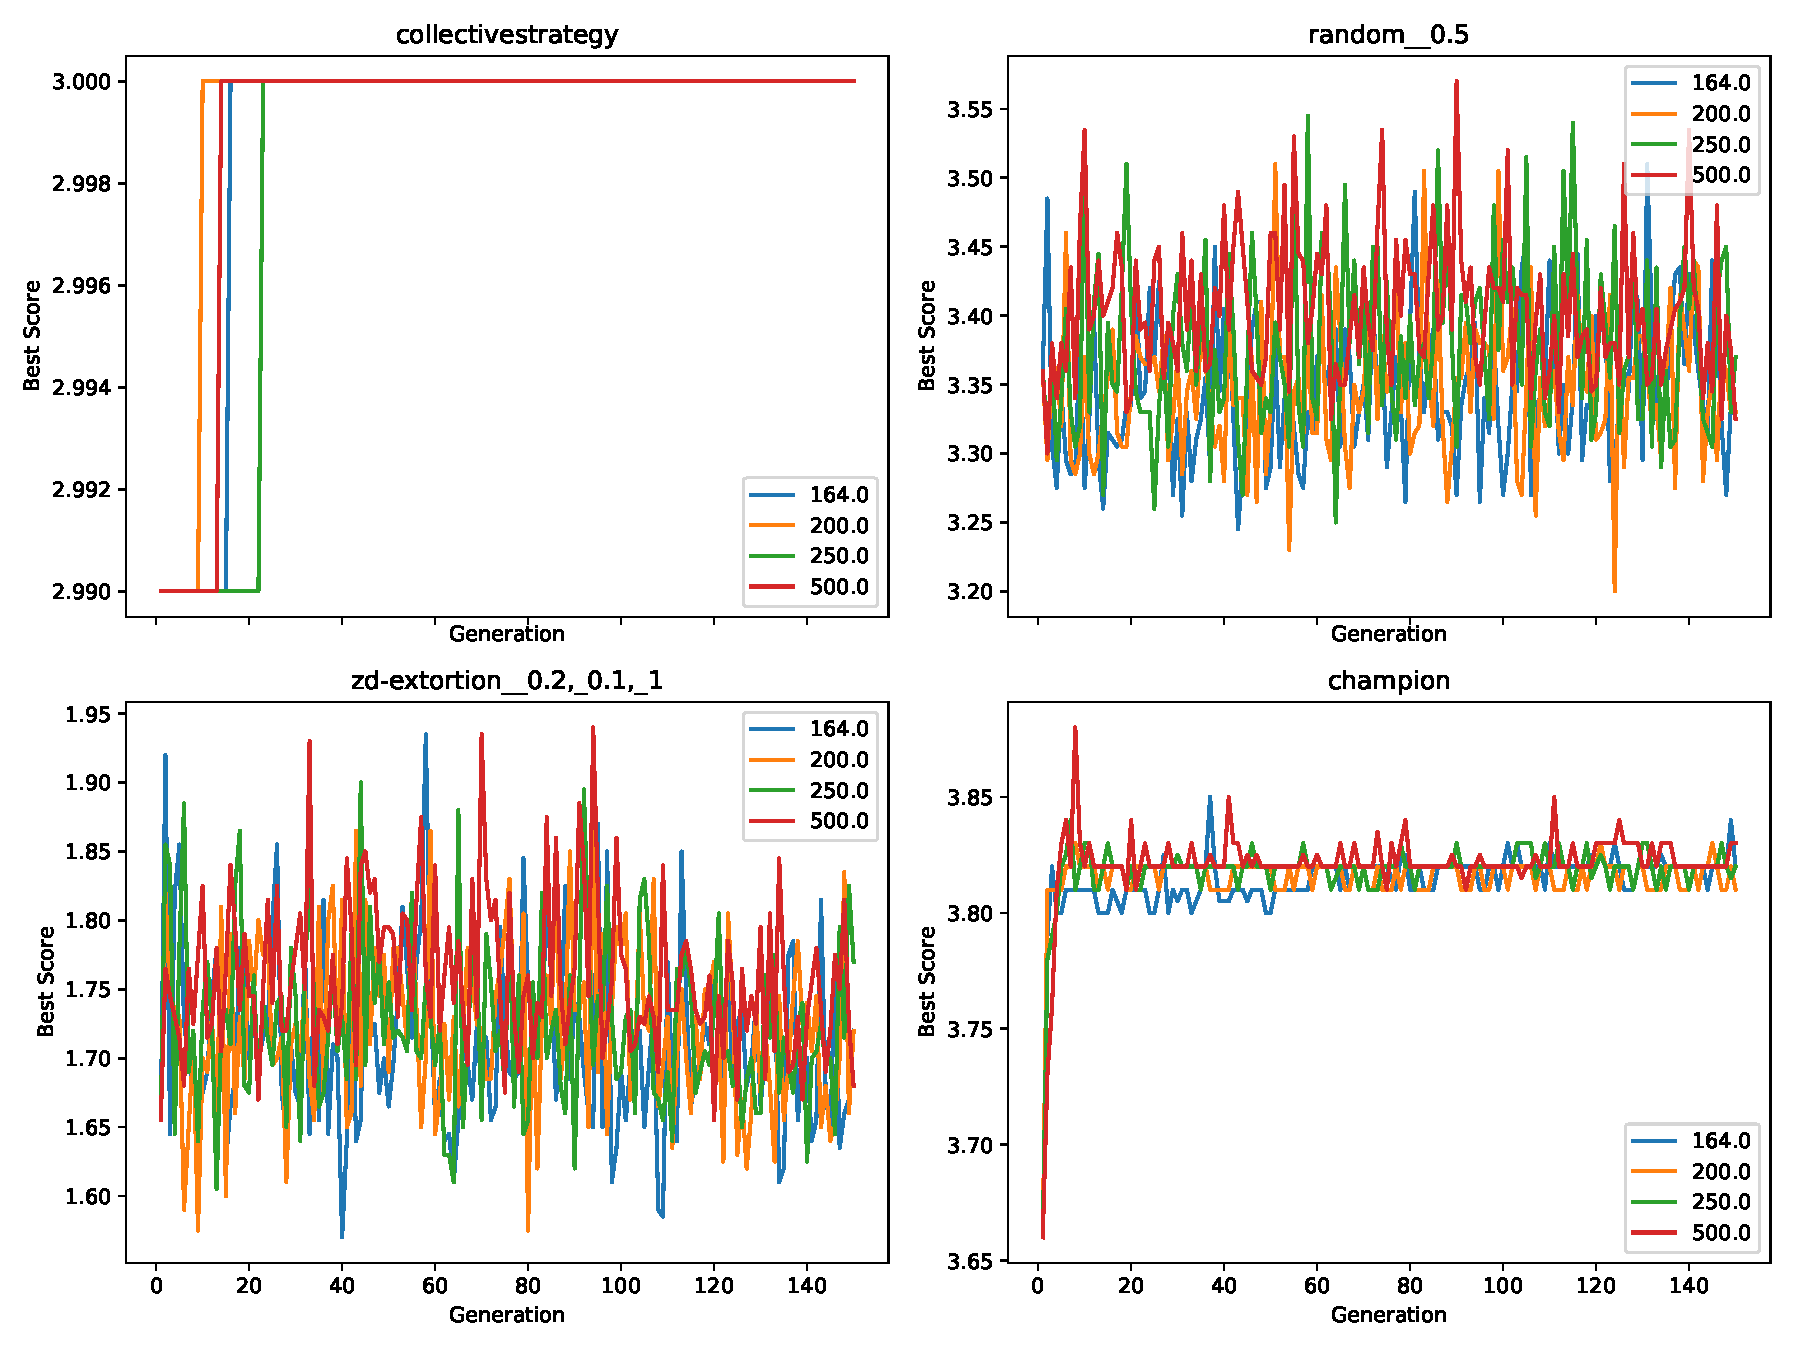
\includegraphics[width=1.0\textwidth, center]{./img/plots/NEW_INIT_POP_bs_v_gen_non_performers.pdf}
    \caption{Non optimal sequence players after changing initial population}\label{fig:NEW-INIT-POP-bs-v-gen-non-performers}
\end{figure}

\subsection{Generation Length}\label{subsec:generationLength}
Figure~\ref{fig:NEW-GEN-bs-v-gen-all} shows the results from changing the number of generations the algorithm will run to \(G \in [50,150,250,350,450,500] \) whilst also running with a population size of \(|P|=200\).

\begin{figure}[ht]
    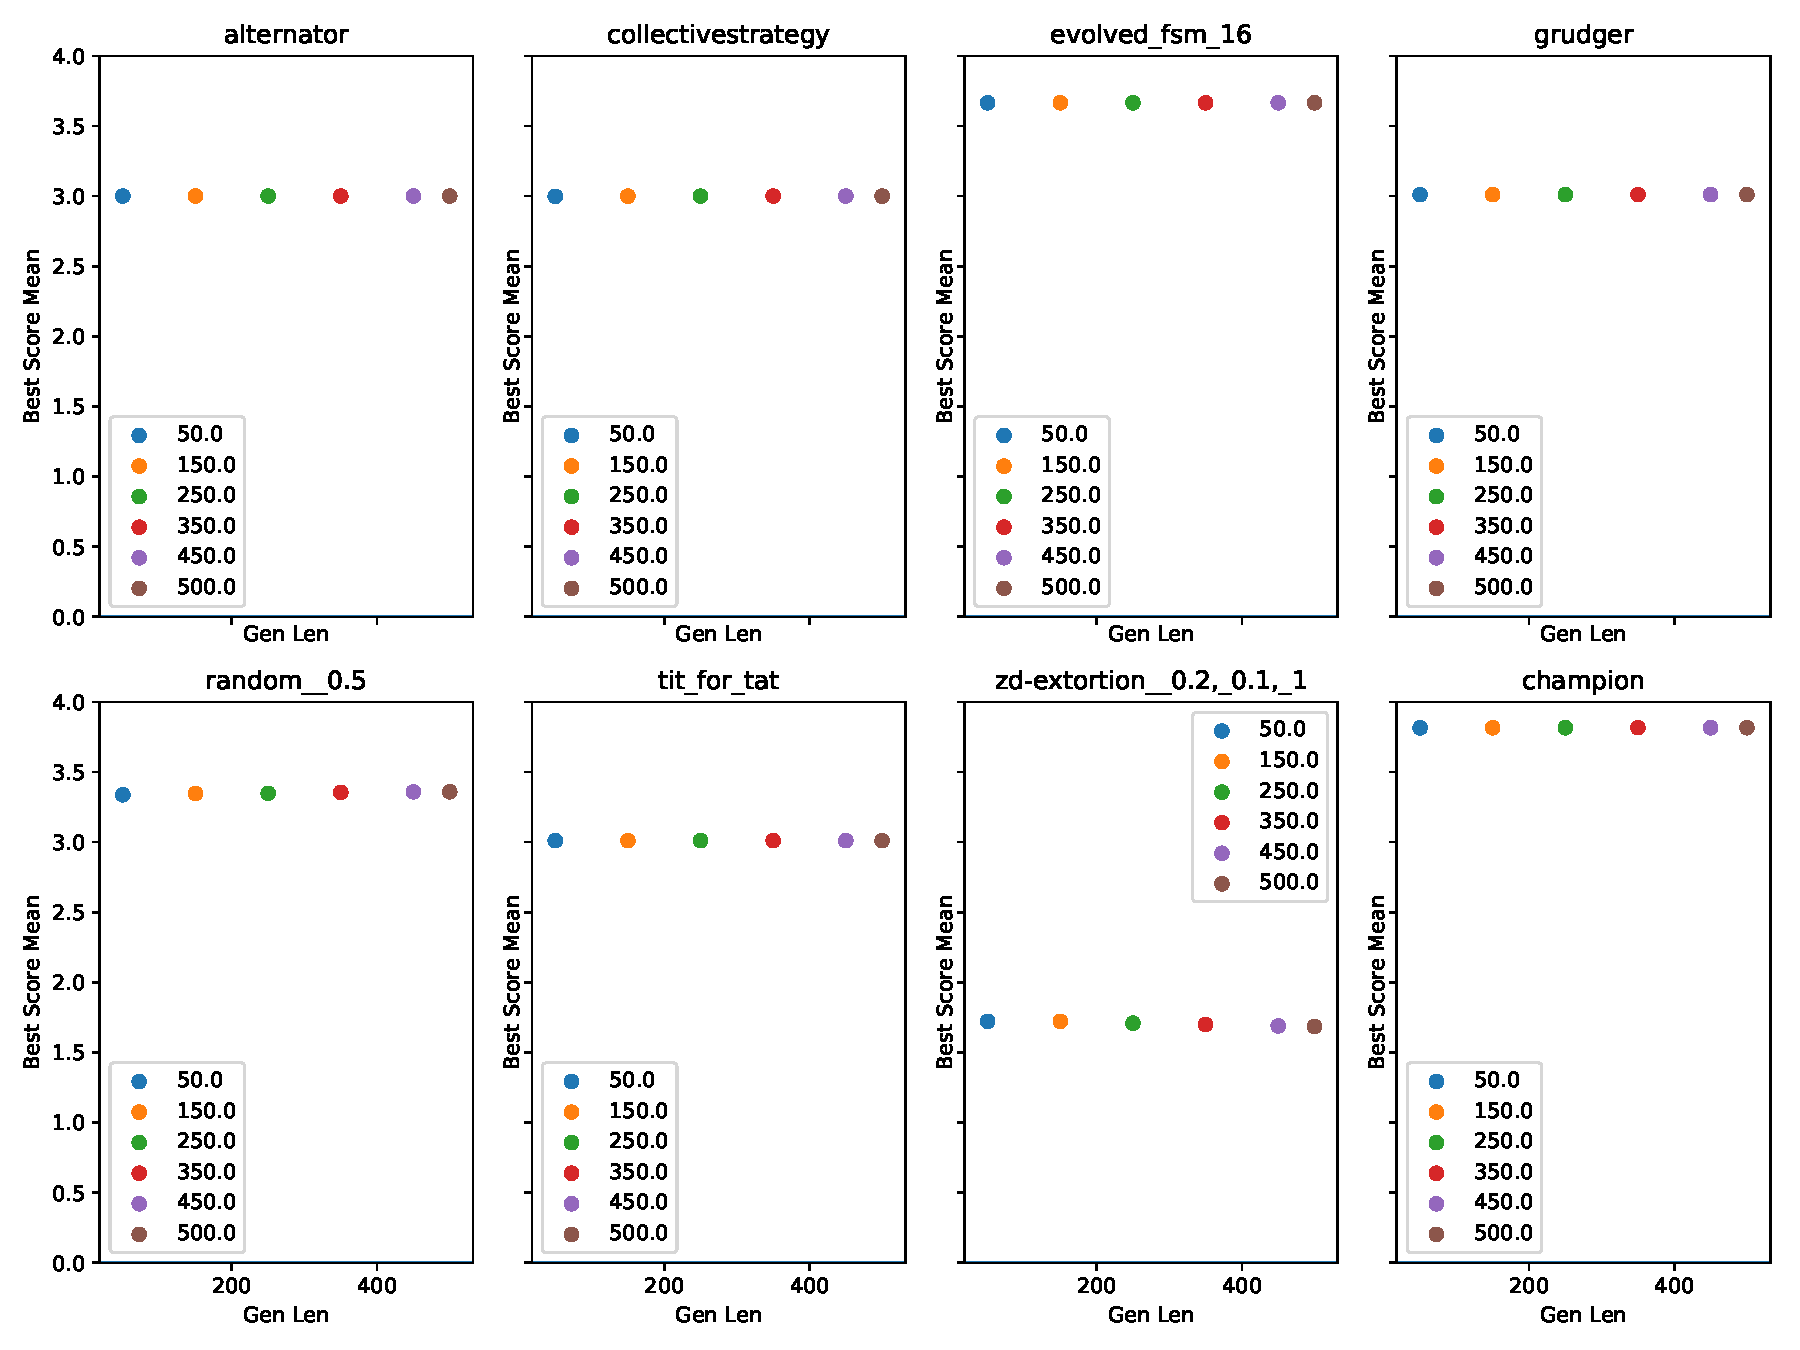
\includegraphics[width=1.0\textwidth, center]{./img/plots/NEW_GEN_bs_v_gen_all.pdf}
    \caption{}\label{fig:NEW-GEN-bs-v-gen-all}
\end{figure}

The Figure~\ref{fig:NEW-GEN-bs-v-gen-all} shows no real improvement from increasing the generations, we will use the results from analysis above sections for constructing the full analysis.

\subsection{Mutation Potency}\label{subsec:mutationPotency}
Figure~\ref{fig:NEW-MUT-POT-bs-v-gen-all} shows the results from changing mutation potency the algorithm will use to be \(M_p \in [1,2,3,5,10,15,20] \) whilst also running with a population size of \(|P|=200\).

\begin{figure}[ht]
    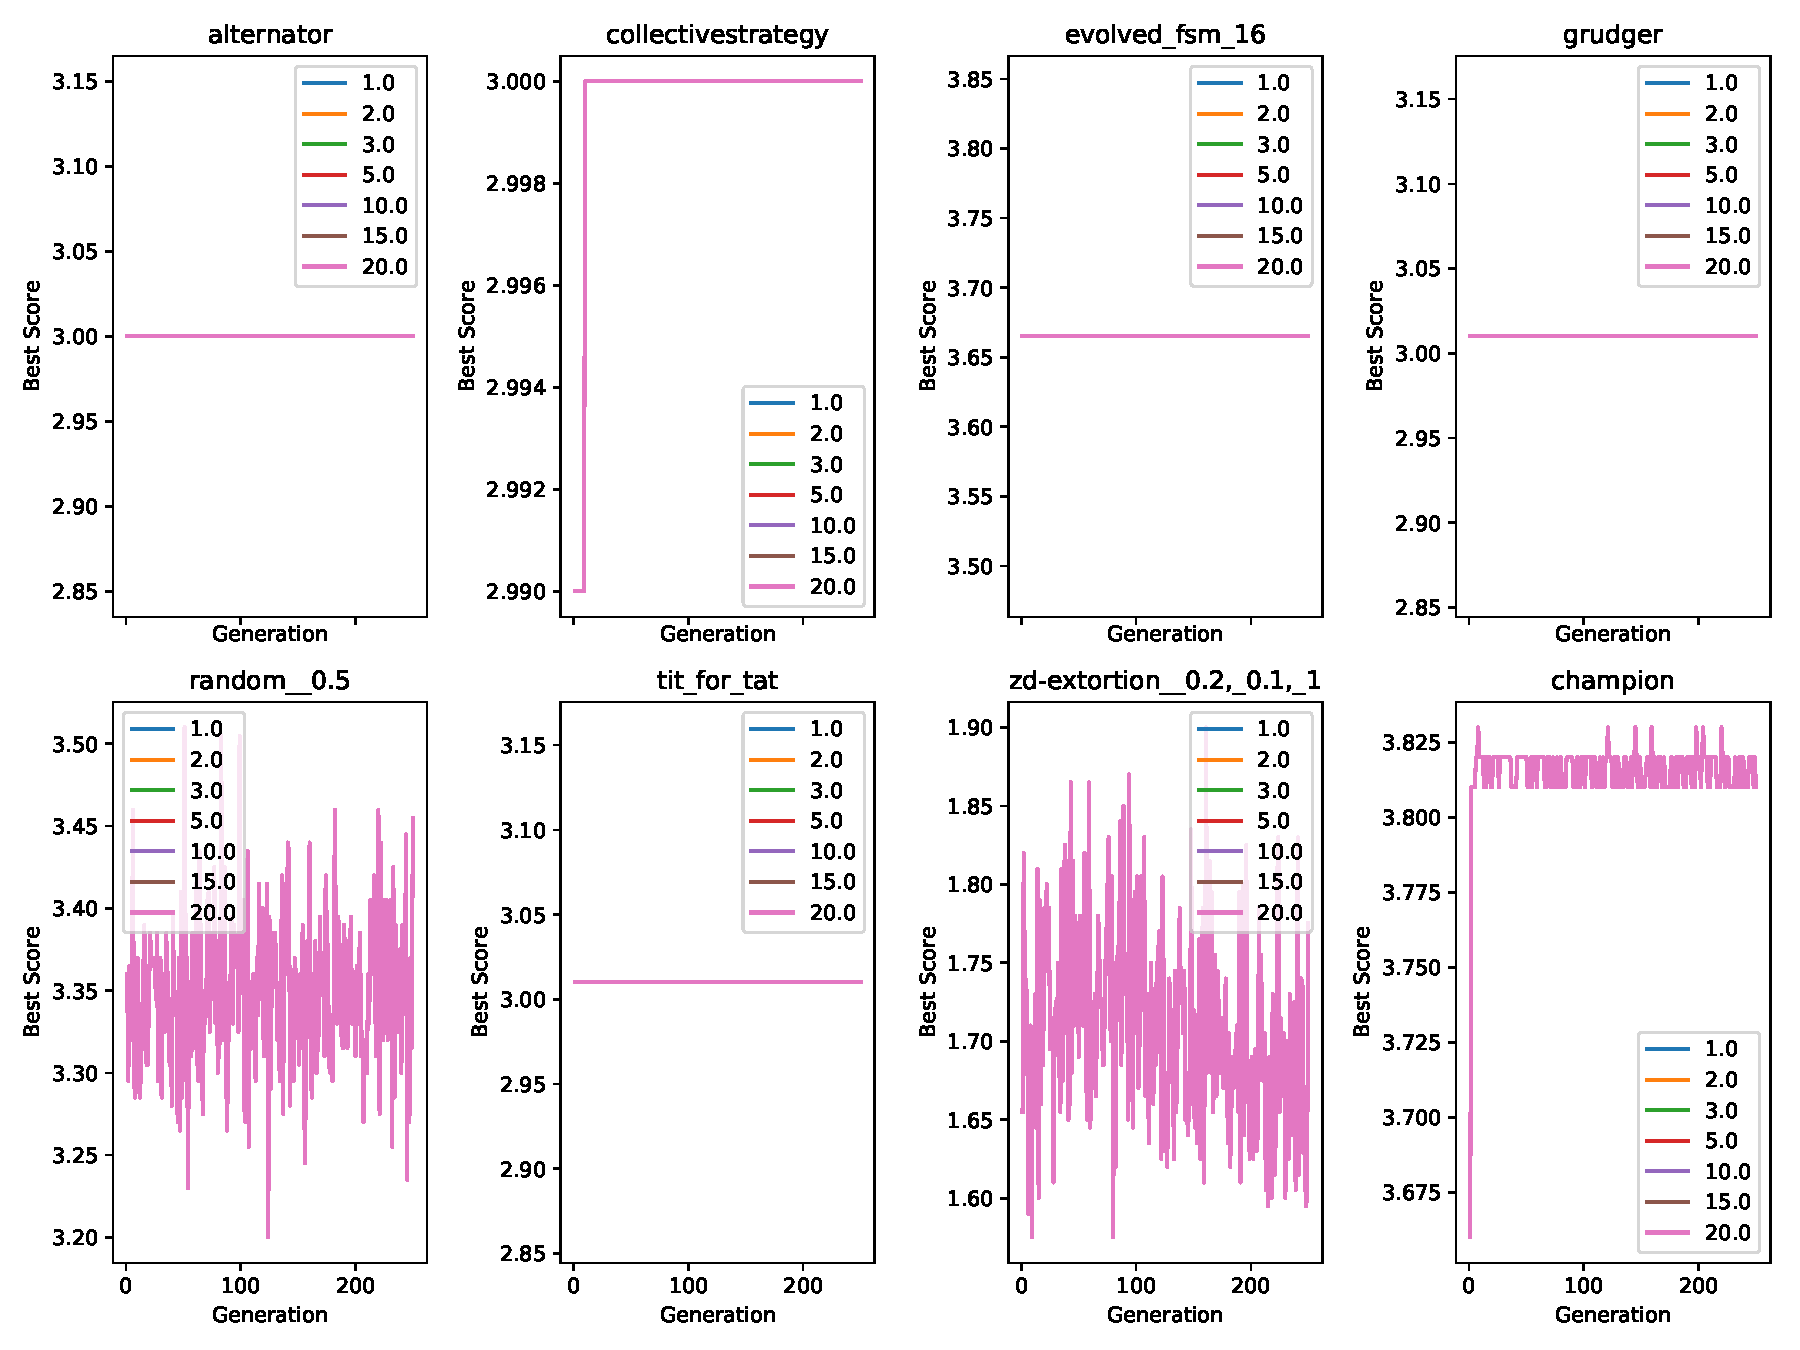
\includegraphics[width=1.0\textwidth, center]{./img/plots/NEW_MUT_POT_bs_v_gen_all.pdf}
    \caption{}\label{fig:NEW-MUT-POT-bs-v-gen-all}
\end{figure}

The Figure~\ref{fig:NEW-MUT-POT-bs-v-gen-all} shows no real improvement from increasing this variable of the algorithm, we will use the results from analysis in previous sections for constructing the full analysis.

\subsection{Mutation Frequency}\label{subsec:mutationFrequency}
Figure~\ref{fig:NEW-MUT-FREQ-bs-gen-all} shows the results from changing mutation potency the algorithm will use to be \(M_f \in [0.1,0.15,0.2,0.25] \) whilst also running with a population size of \(|P|=200\).

\begin{figure}[ht]
    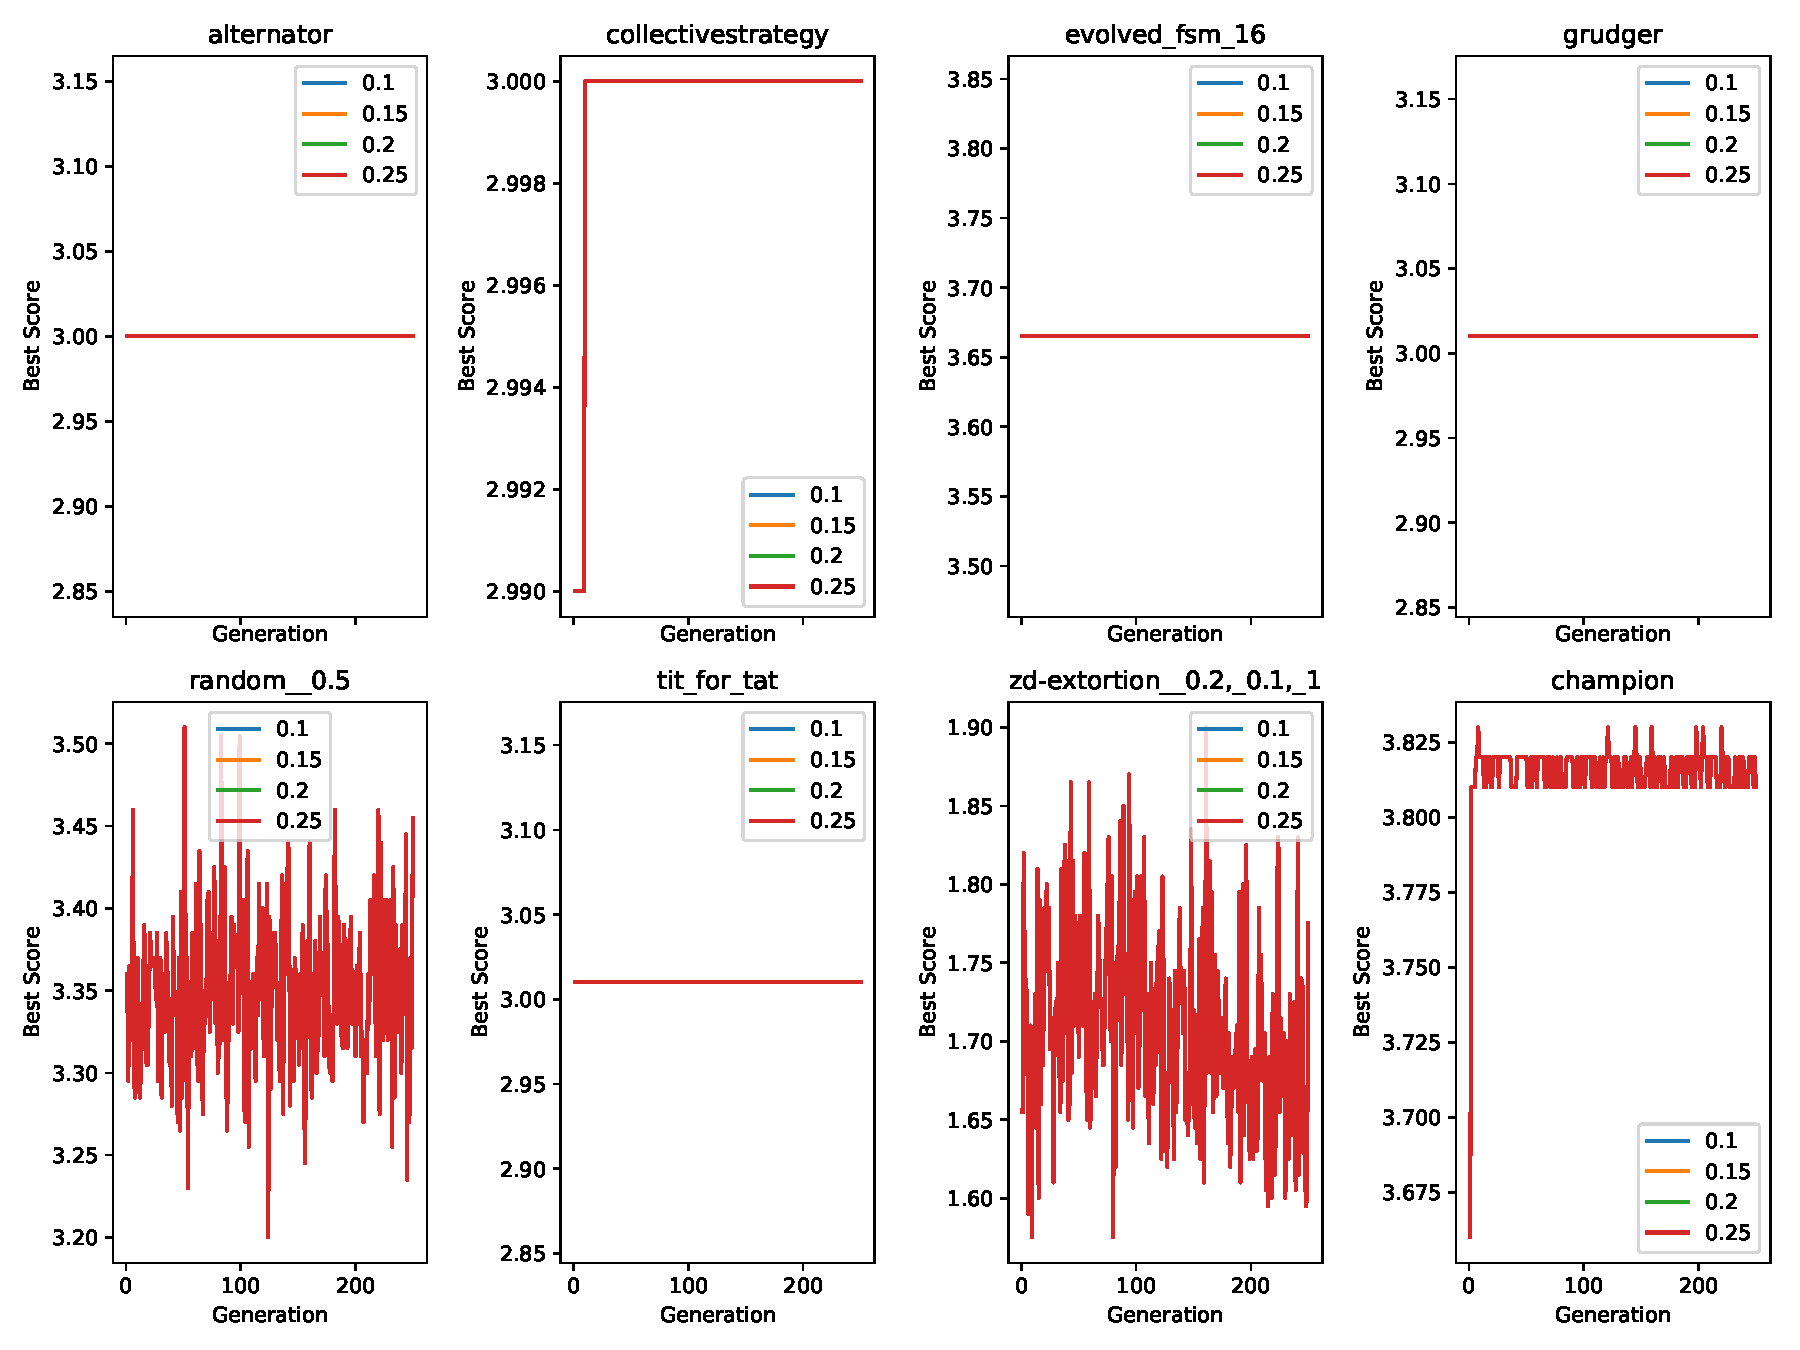
\includegraphics[width=1.0\textwidth, center]{./img/plots/NEW_MUT_FREQ_bs_v_gen_all.pdf}
    \caption{}\label{fig:NEW-MUT-FREQ-bs-gen-all}
\end{figure}

The Figure~\ref{fig:NEW-MUT-FREQ-bs-gen-all} shows no real improvement from increasing this variable of the algorithm, we will use the results from analysis in previous sections for constructing the full analysis.

\subsubsection{Discussion}\label{subsubsec:discussion}
The approach of adding a predefined set of members to the population before running the algorithm was incredibly successful.
We have seen that for most opponents the solution sequence were looking for is given almost immediately.
This result will mean that when calculating the solution sequence for the main population the predefined set, generated by Snippet~\ref{code:initialPopulationCode}, will be used to shorten analysis times.

Opponents such as Random, ZDExtort and Champion are showing that they're not finding the optimal solution.
This is due to the fact these player belong to the class of stochastic opponents.
Section~\ref{sec:stochasticOpponents} will look into these in more detail, putting forward possible approaches to simplify `solving' these opponents.

\section{Stochastic Opponents}\label{sec:stochasticOpponents}
Stochastic opponents form a problem with respect to continuity.
The algorithm we're using continues to generate a new opponent sequence for every generation we run.
This, essentially, leads to the algorithm playing a new version of the opponent every time, leaving very little opportunity to identify features which can be exploited.

The concept of a stochastic opponent can be somewhat `overridden' by seeding the psudo random number generator that creates the parameters that define what moves our opponent will take.
Currently the only way of doing this is by seeing the whole Axelrod library upon initialising the opponent instance, Snippet~\ref{code:wrappingFunction} shows the code for wrapping any given opponent with the global seed command.

\begin{figure}
    \inputminted{python}{code_snippets/classWrappingFunction.py}
    \caption{A function for wrapping a player with a global seed function call}\label{code:wrappingFunction}
\end{figure}

When calculating the sequence solution for all of the opponents we will do so with seeded versions of the stochastic opponents.
The parameters for stochastic opponents will be the default set by the creators and new instances will be made for any variations with real world applications.
For example, default Random players will have a 0.5 chance of playing a C move;
this parameter can optionally be changed, and will for certain opponents.

\section{Conclusion of approach}\label{sec:conclusionOfApproach}